\chapter{Design and implementation}\label{sec:impl}

In order to unroll a loop with non-static bounds, this thesis follows a specific approach:
First, we check whether we are able to unroll the loop.
\Cref{sec:impl:unrollability} describes the conditions necessary and how we check them.
If we determine a loop to be unrollable, we will unroll it with the unrolling process covered in \cref{sec:impl:unroll}.
Once this process is complete, the loop condition of the unrolled loop will be adapted to make sure it runs less than or equal times compared to the original loop.
This is described in~\cref{sec:impl:fixup:header-cond}.
After that, we will create the \textit{fixup code}\footnote{The term \textit{fixup code} describes that code that has to be added to account for cases where the number of times the loop is executed modulo the unrolling factor is not equal to zero.}
, as described in \cref{sec:impl:fixup}.

It is to be noted that in terms of actually implementing this procedure, we will create the fixup code \textit{before} unrolling the loop.
While this order seems counter-intuitive, we chose it in order to simplify loop duplication, as described in~\cref{sec:impl:fixup:loop}.


Henceforth, we assume loops to be in the form of the loop shown in~\cref{fig:impl:general-loop}.
In the reference loop \textit{cmp} refers to a comparison that can be one of the following: $<, >, \geq, \leq$.
Further, $I \in \mathbb{Z}$ refers to the starting value, $N \in \mathbb{Z}$ to the bound, and $c \in \mathbb{Z} \backslash \zeroset$ \label{sec:impl::def-c} to the increment\footnote{N.B.: $c$ may be negative and could hence also be a decrement} of such a loop.
We select this form in view of the fact that most loops follow the form of using a counter or iterating over a given container, which condenses down to this form.
Furthermore, this form allows for many arithmetic properties to be used, as seen in~\cref{sec:impl:unroll}.

\begin{figure}[H]
    \centering
    \begin{algorithmic}
        \Function{Foo}{$I \in \mathbb{Z}, N \in \mathbb{Z}, c \in \mathbb{Z}$}
            \State $i \gets I$
            \While{$i~\text{cmp}~N$}
                \State \Call{DoSomething}{}
                \State $i \gets i + c$
            \EndWhile
        \EndFunction
    \end{algorithmic}
    \caption{A general form of loop starting at $I$ and counting in increments of $c$ up to $N$}
    \label{fig:impl:general-loop}
\end{figure}

\newpage

\section{Determining unrollability}\label{sec:impl:unrollability}

Given that the primary goal of any optimization is to conserve semantics, most optimizations are based upon assumptions.
These assumptions will be assured, by checking corresponding preconditions before the optimization is applied, to ensure that its transformed product will be semantically equivalent.

In the case of loop unrolling, in~\cref{fig:impl:general-loop} we laid out the structured of the targeted loops.
This section formalizes these requirements and extends them, such that the further unrolling process conserves semantics.

Firstly, in view of the fact that we use the existing loop unrolling functionality as a sub-step (see~\cref{sec:impl:unroll}), it needs to be ensured that the respective~\libFIRM-graph is in LCSSA form.
We accomplish this by using the existing mechanics~\cite{aebi18bachelorarbeit}.
While it is a preliminary step, assuring LCSSA form can never be a hindrance to unrolling, since it is possible to convert any given graph into LCSSA.
Due to the restrictions of the existing loop unrolling mechanism, a loop must also be the innermost loop, meaning it does not have any nested loops inside of it.
Nested loops inherently cause larger code sizes and hardly saves jumps, since most jumps will occur in the inner loops.
Therefore, the restriction will in practice most likely not harm performance.
\Cref{sec:impl:sel-factor} describes the mechanics for determining if and how a given loop should be unrolled based on size.

Moreover, in order for loops to be in the form described in \cref{sec:impl}, loops have to have a header, which itself controls the control flow by comparing a counter to a bound, using any of the four allowed comparison types.
The header is the only point in the loop from which the loop can exit; meaning there are no conditionals in the body that allow the control flow to leave the loop.
This primarily requires there not to be any \texttt{break}-like structures.

Seeing that there is an explicit entry point for the loop, the header, there are no preconditions for $I$, since it is therefore only evaluate once in a block dominating the header, but inherently not determining of the control flow after the initial evaluation.
On the contrary, $N$, the bound, has to be loop-invariant, which means that it may not change through the entire evaluation of the loop, because it is checked against $i$ in every iteration.
As an example, consider a loop, such as the one in \cref{fig:impl:general-loop}, replacing \texttt{DoSomething} with \texttt{$N =$ randomNumber}.
If we now execute the body $f > 1$ times consecutively, we will effectively lose $f - 1$ checks.
Assume that initially $I = 0, c = 1, f = 2, N = 2$, and assume in the first execution in the loop body $N$ is set to $0$ by chance, whereas in the second iteration it is set to $7$.
Now given that when unrolling the condition is removed for the entering the second body, the loop body would at least four times, which does not conserve semantics, as it should only be executed once.
Concluding, only if $N$ is loop-invariant, the bound checks can be performed less often, while keeping the original semantics intact.

If $N$ is constant it is obviously loop-invariant, but what if it is the result of a function call or of a load from memory?
For the case that $N$ is function call, this function call must be pure (i.e., not have any side-effects), and only have loop-invariant arguments, seeing that the call is then by definition loop-invariant itself.

In case that $N$ is being loaded from memory, stricter conditions have to be met.
All stores within the loop must be sure not to alias the memory location of $N$.
Further, any calls must either invoke functions known at compile time and none of these may contain aliasing stores or have aliasing parameters.
Otherwise, the loop cannot be unrolled with a loaded bound, due to these called functions potentially modifying $N$.

Lastly, the unroll-factor -- meaning how often the loop body is copied inside the unrolled loop -- $f$ is selected (see \cref{sec:impl:sel-factor} and hence known at compile time.
We can therefore restrict the increment $c$, such that $t_{min} \leq c \cdot (f+1) \leq t_{max}$, where $t_{min}$ is the minimum value of the integer type of $c$ and $t_{max}$ the respective maximum.
Hence, we prevent $c \cdot (f + 1)$ from overflowing, which will turn out to be important in \cref{sec:impl:fixup:header-cond} and \cref{sec:impl:fixup:duff}, and further discussed there.
In order to assure this property, we have to force $c$ to be a compile-time constant (which inherently is loop invariant).
Even though the restrictions on $c$ seem comparatively tight, in real-world code (gcc, \texttt{spec2006}) only approximately $1.2\%$ of loops that meet the previous conditions are not unrollable because of the restriction that  $t_{min} \leq c \cdot (f+1) \leq t_{max}$.

It is worth mentioning that the unrollability with the method above is only checked if the current loop unrolling mechanism~\cite{aebi18bachelorarbeit} determines that the current unrolling process cannot be applied.
We chose this design, for the reason that statically unrolling without any further fixup code inherently simplifies the control flow and hence should yield better, or (at least) equal, performance.

\section{Unrolling}\label{sec:impl:unroll}

To get started with unrolling loops that have unknown bounds, we unroll them by a given factor without considering whether the transformation is semantically invariant.
Semantic equivalence, which is broken due to the failure to consider how the factor relates to the original amount of iterations, will be restored in \cref{sec:impl:fixup}.

\libFIRM{} already provides an unrolling mechanism for unrolling a loop with a given factor $f$~\cite{aebi18bachelorarbeit}.\footnote{N.B.: All following operations preserve the LCSSA property of the code.}
In order to avoid code duplication, we will use be utilizing this solution.

Further, figures~\ref{fig:impl:unroll:unroll-factor-2-before}~and~\ref{fig:impl:unroll:unroll-factor-2-after} show a firm graph of a loop that is to be unrolled or is unrolled using a factor of two, respectively.
Especially to be noted is that in \cref{fig:impl:unroll:unroll-factor-2-after} we duplicate the loop header, and that hence the number of conditional jumps did not decrease through the loop unroll.
With the previous usage, this was not an issue, because~\libFIRM{} would automatically remove these excess headers~\cite{aebi18bachelorarbeit} using its constant bit analysis.
Unfortunately though in the use cases of an unknown bound, the constant bit analysis does not suffice.
This is due to the fact that the additional semantics, meaning that we are sure not to have to exit the unrolled loop from its body at any time, that are implicitly affixed to the transformed loop, cannot be recognized by~\libFIRM.
Therefore, the need to manually prune the graph to remove the excess headers arises.
\Cref{alg:impl:unroll:prune-headers} shows the algorithm used to accomplish this.
First, we rewire all $\Phi$-nodes in the excess header, such that all in-loop nodes depending on any given $\Phi$-node each get the in-loop predecessors of the $\Phi$-node as predecessors themselves, while the $\Phi$-node falls into desuetude.
We apply the same transformations to the descendants of the block itself.

\begin{algorithm}
    \begin{algorithmic}
        \Function{PruneExcessHeader}{$copiedHeader: \text{Block}$}
            \ForAll{$phi \in copiedHeader$}
                \State \Call{PrunePhi}{$phi, copiedHeader$}
            \EndFor
            \ForAll{$post \in copiedHeader.descendants$}
                \State $post.predecessors \gets (post.predecessors \backslash \{copiedHeader\}) \cup \newline \{b \vert  b \in copiedHeader.predecessors, b.loop = copiedHeader.loop\}$
            \EndFor
        \EndFunction
        \State{}
        \Function{PrunePhi}{$phi: \Phi \text{-node}, copiedHeader: \text{Block}$}
            \ForAll{$out \in phi.descendants$}
                \State \Comment $out$ is ensured to be $\Phi$-node by the LCSSA construction algorithm~\cite{aebi18bachelorarbeit}
                \If{$out.block \neq copiedHeader$}
                    \State $out.predecessors \gets (out.predecessors \backslash \{phi\}) \cup \newline \{n \vert  n \in phi.predecessors, n.loop = out.loop\}$
                \EndIf
            \EndFor
        \EndFunction
    \end{algorithmic}
    \caption{Pruning excess headers after unrolling}
    \label{alg:impl:unroll:prune-headers}
\end{algorithm}

\begin{algorithm}[h]
    \begin{algorithmic}
        \Function{UnrollExisting}{$factor: \mathbb{N}_{> 1}, loop: \text{Loop}$}
            \State \Call{AssureLCSSA}{$loop$}
            \ForAll{$block \in loop$}
                \For{$i \in \{1..(factor - 1)\}$}
                    \State \Call{DuplicateBlock}{$block$}
                \EndFor
            \EndFor
            \State \Call{RewireDuplicatedBlocks}{} \Comment{Attach blocks to form unrolled structure}
            \State \Comment{$loop$ is still in LCSSA form after unrolling}
        \EndFunction
    \end{algorithmic}
    \caption{Pseudo-code for the existing unrolling mechanism~\cite{aebi18bachelorarbeit}}
    \label{fig:impl:unroll:existing-mechanism}
\end{algorithm}

\begin{figure}[H]
    \centering
    \begin{adjustbox}{max width=\textwidth}
        \centering
        % Scale factor 0.024395857307249712
\definecolor{color0}{RGB}{222,239,234}
\definecolor{color1}{RGB}{192,192,192}
\definecolor{color2}{RGB}{153,153,255}
\definecolor{color3}{RGB}{255,153,153}
\definecolor{color4}{RGB}{255,255,255}
\definecolor{color5}{RGB}{255,255,153}
\definecolor{color6}{RGB}{153,255,153}
\definecolor{color7}{RGB}{0,150,60}
\definecolor{color8}{RGB}{170,30,30}
\definecolor{color9}{RGB}{255,0,0}
\definecolor{color10}{RGB}{100,100,255}
\definecolor{color11}{RGB}{0,0,0}
\definecolor{color12}{RGB}{128,0,128}
% Bounding Box: 968.0, 869.0
\begin{tikzpicture}
	\node[fill=color0, draw, minimum width=17.40644418872267cm, minimum height=8.611737629459148cm] (n1) at (14.895584286649068cm ,-2.427387802071346cm) {};
	% 1 node layouts
	\node[scale=0.8871220838999895, transform shape] at (14.895584286649068cm ,1.599834579976985cm) {Block  227};
	\node[fill=color0, draw, minimum width=9.73825221688215cm, minimum height=8.855696202531645cm] (n2) at (5.601001827658567cm ,7.282163406214039cm) {};
	% 1 node layouts
	\node[scale=0.8871220838999895, transform shape] at (5.601001827658567cm ,11.431365074798618cm) {Block  217};
	\node[fill=color1, draw, minimum width=23.5988063810104cm, minimum height=21.2cm] (n3) at (12.165341050113947cm ,3.5008055235903335cm) {};
	% 1 node layouts
	\node[scale=0.8871220838999895, transform shape] at (12.165341050113947cm ,13.822159090909091cm) {\#LOOP-6};
	\node[fill=color2, draw, minimum width=2.342002301495972cm, minimum height=0.7318757192174914cm] (n4) at (2.312583767684289cm ,8.709321058688147cm) {};
	% 1 node layouts
	\node[scale=0.8871220838999895, transform shape] at (2.312583767684289cm ,8.709321058688147cm) {Phi[loop]  218};
	\node[fill=color3, draw, minimum width=2.634752589182969cm, minimum height=0.7318757192174914cm] (n5) at (5.761727475800447cm ,3.5861910241657076cm) {};
	% 1 node layouts
	\node[scale=0.8871220838999895, transform shape] at (5.761727475800447cm ,3.5861910241657076cm) {Proj X false 226};
	\node[fill=color3, draw, minimum width=2.53716915995397cm, minimum height=0.7318757192174914cm] (n6) at (8.83560549651391cm ,3.5861910241657076cm) {};
	% 1 node layouts
	\node[scale=0.8871220838999895, transform shape] at (8.83560549651391cm ,3.5861910241657076cm) {Proj X true 225};
	\node[fill=color3, draw, minimum width=1.854085155350978cm, minimum height=0.7318757192174914cm] (n7) at (7.264942801055981cm ,5.293901035673187cm) {};
	% 1 node layouts
	\node[scale=0.8871220838999895, transform shape] at (7.264942801055981cm ,5.293901035673187cm) {Cond  224};
	\node[fill=color4, draw, minimum width=3.5373993095512084cm, minimum height=0.7318757192174914cm] (n8) at (7.264942801055981cm ,7.001611047180667cm) {};
	% 1 node layouts
	\node[scale=0.8871220838999895, transform shape] at (7.264942801055981cm ,7.001611047180667cm) {Cmp b less\_equal 223};
	\node[fill=color5, draw, minimum width=2.9762945914844647cm, minimum height=0.7318757192174914cm] (n9) at (8.149292628443783cm ,8.709321058688147cm) {};
	% 1 node layouts
	\node[scale=0.8871220838999895, transform shape] at (8.149292628443783cm ,8.709321058688147cm) {Const 0x10 Is 222};
	\node[fill=color6, draw, minimum width=1.7565017261219793cm, minimum height=0.7318757192174914cm] (n10) at (5.20349285859338cm ,8.709321058688147cm) {};
	% 1 node layouts
	\node[scale=0.8871220838999895, transform shape] at (5.20349285859338cm ,8.709321058688147cm) {Phi Is 219};
	\node[fill=color5, draw, minimum width=2.781127733026467cm, minimum height=0.7318757192174914cm] (n11) at (6.2984363365599405cm ,10.417031070195627cm) {};
	% 1 node layouts
	\node[scale=0.8871220838999895, transform shape] at (6.2984363365599405cm ,10.417031070195627cm) {Const 0x0 Is 215};
	\node[fill=color7, draw, minimum width=0.48791714614499426cm, minimum height=0.48791714614499426cm] (n12) at (1.3417721518987342cm ,7.001611047180667cm) {};
	\node[fill=color7, draw, minimum width=0.48791714614499426cm, minimum height=0.48791714614499426cm] (n13) at (4.7643674270628855cm ,7.001611047180667cm) {};
	\node[fill=color7, draw, minimum width=0.48791714614499426cm, minimum height=0.48791714614499426cm] (n14) at (2.8005009138292833cm ,10.417031070195627cm) {};
	\node[fill=color7, draw, minimum width=0.48791714614499426cm, minimum height=0.48791714614499426cm] (n15) at (1.824666621539295cm ,10.417031070195627cm) {};
	\node[fill=color7, draw, minimum width=0.48791714614499426cm, minimum height=0.48791714614499426cm] (n16) at (4.175996750829215cm ,10.417031070195627cm) {};
	\node[fill=color7, draw, minimum width=0.48791714614499426cm, minimum height=0.48791714614499426cm] (n17) at (2.3176064441887227cm ,7.001611047180667cm) {};
	\node[fill=color7, draw, minimum width=0.48791714614499426cm, minimum height=0.48791714614499426cm] (n18) at (3.297745887768226cm ,7.001611047180667cm) {};
	\node[fill=color2, draw, minimum width=2.268814729574223cm, minimum height=0.7318757192174914cm] (n19) at (13.047598095624902cm ,-4.537629459148446cm) {};
	% 1 node layouts
	\node[scale=0.8871220838999895, transform shape] at (13.047598095624902cm ,-4.537629459148446cm) {Proj M M 235};
	\node[fill=color2, draw, minimum width=1.6345224395857307cm, minimum height=0.7318757192174914cm] (n20) at (13.047598095624902cm ,-2.8299194476409664cm) {};
	% 1 node layouts
	\node[scale=0.8871220838999895, transform shape] at (13.047598095624902cm ,-2.8299194476409664cm) {Call  234};
	\node[fill=color5, draw, minimum width=3.659378596087457cm, minimum height=0.7318757192174914cm] (n21) at (9.961522146257813cm ,-1.1222094361334867cm) {};
	% 1 node layouts
	\node[scale=0.8871220838999895, transform shape] at (9.961522146257813cm ,-1.1222094361334867cm) {Address \&\_printf P 229};
	\node[fill=color5, draw, minimum width=3.41542002301496cm, minimum height=0.7318757192174914cm] (n22) at (16.011694758455743cm ,-1.1222094361334867cm) {};
	% 1 node layouts
	\node[scale=0.8871220838999895, transform shape] at (16.011694758455743cm ,-1.1222094361334867cm) {Address \&str.0 P 233};
	\node[fill=color2, draw, minimum width=1.5369390103567317cm, minimum height=0.7318757192174914cm] (n23) at (13.047598095624902cm ,-1.1222094361334867cm) {};
	% 1 node layouts
	\node[scale=0.8871220838999895, transform shape] at (13.047598095624902cm ,-1.1222094361334867cm) {Phi  403};
	\node[fill=color3, draw, minimum width=1.6833141542002301cm, minimum height=0.7318757192174914cm] (n24) at (7.3999571289965935cm ,0.585500575373993cm) {};
	% 1 node layouts
	\node[scale=0.8871220838999895, transform shape] at (7.3999571289965935cm ,0.585500575373993cm) {Jmp  240};
	\node[fill=color4, draw, minimum width=1.9272727272727272cm, minimum height=0.7318757192174914cm] (n25) at (20.477007926300555cm ,-2.8299194476409664cm) {};
	% 1 node layouts
	\node[scale=0.8871220838999895, transform shape] at (20.477007926300555cm ,-2.8299194476409664cm) {Add Is 239};
	\node[fill=color5, draw, minimum width=2.781127733026467cm, minimum height=0.7318757192174914cm] (n26) at (21.842304654888423cm ,-1.1222094361334867cm) {};
	% 1 node layouts
	\node[scale=0.8871220838999895, transform shape] at (21.842304654888423cm ,-1.1222094361334867cm) {Const 0x1 Is 238};
	\node[fill=color6, draw, minimum width=1.7565017261219793cm, minimum height=0.7318757192174914cm] (n27) at (19.085572779169205cm ,-1.1222094361334867cm) {};
	% 1 node layouts
	\node[scale=0.8871220838999895, transform shape] at (19.085572779169205cm ,-1.1222094361334867cm) {Phi Is 402};
	\node[fill=color7, draw, minimum width=0.48791714614499426cm, minimum height=0.48791714614499426cm] (n28) at (13.047598095624902cm ,0.585500575373993cm) {};
	\node[fill=color7, draw, minimum width=0.48791714614499426cm, minimum height=0.48791714614499426cm] (n29) at (19.085572779169205cm ,0.585500575373993cm) {};
	\node[fill=color7, draw, minimum width=0.48791714614499426cm, minimum height=0.48791714614499426cm] (n30) at (13.047598095624902cm ,-6.123360184119678cm) {};
	\node[fill=color7, draw, minimum width=0.48791714614499426cm, minimum height=0.48791714614499426cm] (n31) at (20.477007926300555cm ,-4.537629459148446cm) {};
	\node[fill=color8, draw, minimum width=0.48791714614499426cm, minimum height=0.48791714614499426cm] (n32) at (5.1228908594508cm ,12.929804372842348cm) {};
	\node[fill=color8, draw, minimum width=0.48791714614499426cm, minimum height=0.48791714614499426cm] (n33) at (7.3999571289965935cm ,-1.1222094361334867cm) {};
	\draw[color=color9, -latex] (14.895584286649068cm ,1.8784810126582279cm) -- (14.895584286649068cm ,2.366398158803222cm) -- (8.83560549651391cm ,2.366398158803222cm) -- (8.83560549651391cm ,3.220253164556962cm);
	\node[] at (15.090751145107065cm ,2.2337456846950516cm) {
		\scalebox{0.8871220838999895}{0}
	};
	\draw[color=color10, -latex] (2.8980843430582826cm ,9.075258918296893cm) -- (2.8980843430582826cm ,9.563176064441887cm) -- (2.8005009138292833cm ,9.563176064441887cm) -- (2.8005009138292833cm ,10.17307249712313cm);
	\node[] at (3.09325120151628cm ,9.430523590333717cm) {
		\scalebox{0.8871220838999895}{0}
	};
	\draw[color=color10, -latex] (1.7270831923102963cm ,9.075258918296893cm) -- (1.7270831923102963cm ,9.563176064441887cm) -- (1.824666621539295cm ,9.563176064441887cm) -- (1.824666621539295cm ,10.17307249712313cm);
	\node[] at (1.9222500507682938cm ,9.430523590333717cm) {
		\scalebox{0.8871220838999895}{1}
	};
	\draw[color=color9, -latex] (5.761727475800447cm ,3.9521288837744533cm) -- (5.761727475800447cm ,4.440046029919448cm) -- (6.801421512218236cm ,4.440046029919448cm) -- (6.801421512218236cm ,4.927963176064441cm);
	\node[] at (5.956894334258444cm ,4.307393555811277cm) {
		\scalebox{0.8871220838999895}{0}
	};
	\draw[color=color9, -latex] (8.83560549651391cm ,3.9521288837744533cm) -- (8.83560549651391cm ,4.440046029919448cm) -- (7.728464089893725cm ,4.440046029919448cm) -- (7.728464089893725cm ,4.927963176064441cm);
	\node[] at (9.030772354971909cm ,4.307393555811277cm) {
		\scalebox{0.8871220838999895}{0}
	};
	\draw[color=color11, -latex] (7.264942801055981cm ,5.659838895281933cm) -- (7.264942801055981cm ,6.635673187571921cm);
	\node[] at (7.460109659513979cm ,6.128029703682393cm) {
		\scalebox{0.8871220838999895}{0}
	};
	\draw[color=color11, -latex] (6.380592973668179cm ,7.367548906789413cm) -- (6.380592973668179cm ,7.855466052934407cm) -- (5.642618290123875cm ,7.855466052934407cm) -- (5.642618290123875cm ,8.343383199079401cm);
	\node[] at (6.5757598321261765cm ,7.722813578826237cm) {
		\scalebox{0.8871220838999895}{0}
	};
	\draw[color=color11, -latex] (8.149292628443783cm ,7.367548906789413cm) -- (8.149292628443783cm ,8.343383199079401cm);
	\node[] at (8.34445948690178cm ,7.835739715189873cm) {
		\scalebox{0.8871220838999895}{1}
	};
	\draw[color=color11, -latex] (5.642618290123875cm ,9.075258918296893cm) -- (5.642618290123875cm ,9.563176064441887cm) -- (6.2984363365599405cm ,9.563176064441887cm) -- (6.2984363365599405cm ,10.051093210586881cm);
	\node[] at (5.837785148581872cm ,9.430523590333717cm) {
		\scalebox{0.8871220838999895}{0}
	};
	\draw[color=color11, -latex] (4.7643674270628855cm ,9.075258918296893cm) -- (4.7643674270628855cm ,9.563176064441887cm) -- (4.175996750829215cm ,9.563176064441887cm) -- (4.175996750829215cm ,10.17307249712313cm);
	\node[] at (4.959534285520883cm ,9.430523590333717cm) {
		\scalebox{0.8871220838999895}{1}
	};
	\draw[color=color10, -latex] (1.3417721518987342cm ,7.245569620253164cm) -- (1.3417721518987342cm ,7.855466052934407cm) -- (1.5319163338522985cm ,7.855466052934407cm) -- (1.5319163338522985cm ,8.343383199079401cm);
	\node[] at (1.5369390103567317cm ,7.661823935558113cm) {
		\scalebox{0.8871220838999895}{0}
	};
	\draw[color=color11, -latex] (4.7643674270628855cm ,7.245569620253164cm) -- (4.7643674270628855cm ,8.343383199079401cm);
	\node[] at (4.959534285520883cm ,7.713760428653624cm) {
		\scalebox{0.8871220838999895}{0}
	};
	\draw[color=color10, -latex] (2.3176064441887227cm ,7.245569620253164cm) -- (2.312583767684289cm ,8.343383199079401cm);
	\node[] at (2.5116432004332228cm ,7.713760428653624cm) {
		\scalebox{0.8871220838999895}{0}
	};
	\draw[color=color12, -latex] (3.297745887768226cm ,7.245569620253164cm) -- (3.297745887768226cm ,7.855466052934407cm) -- (3.09325120151628cm ,7.855466052934407cm) -- (3.09325120151628cm ,8.343383199079401cm);
	\node[] at (3.4929127462262235cm ,7.661823935558113cm) {
		\scalebox{0.8871220838999895}{1}
	};
	\draw[color=color10, -latex] (13.047598095624902cm ,-4.171691599539701cm) -- (13.047598095624902cm ,-3.195857307249712cm);
	\node[] at (13.242764954082899cm ,-3.7035007911392404cm) {
		\scalebox{0.8871220838999895}{0}
	};
	\draw[color=color10, -latex] (13.047598095624902cm ,-2.4639815880322207cm) -- (13.047598095624902cm ,-1.4881472957422324cm);
	\node[] at (13.242764954082899cm ,-1.9957907796317607cm) {
		\scalebox{0.8871220838999895}{0}
	};
	\draw[color=color11, -latex] (12.502757282429657cm ,-2.4639815880322207cm) -- (12.502757282429657cm ,-1.9760644418872266cm) -- (9.961522146257813cm ,-1.9760644418872266cm) -- (9.961522146257813cm ,-1.4881472957422324cm);
	\node[] at (12.697924140887656cm ,-2.108716915995397cm) {
		\scalebox{0.8871220838999895}{1}
	};
	\draw[color=color11, -latex] (13.592438908820146cm ,-2.4639815880322207cm) -- (13.592438908820144cm ,-1.9760644418872266cm) -- (16.011694758455743cm ,-1.9760644418872266cm) -- (16.011694758455743cm ,-1.4881472957422324cm);
	\node[] at (13.787605767278144cm ,-2.108716915995397cm) {
		\scalebox{0.8871220838999895}{2}
	};
	\draw[color=color10, -latex] (13.047598095624902cm ,-0.7562715765247411cm) -- (13.047598095624902cm ,0.34154200230149595cm);
	\node[] at (13.242764954082899cm ,-0.2880807681242808cm) {
		\scalebox{0.8871220838999895}{0}
	};
	\draw[color=color11, -latex] (19.99518974448237cm ,-2.4639815880322207cm) -- (19.99518974448237cm ,-1.9760644418872266cm) -- (19.085572779169205cm ,-1.9760644418872266cm) -- (19.085572779169205cm ,-1.4881472957422324cm);
	\node[] at (20.19035660294037cm ,-2.108716915995397cm) {
		\scalebox{0.8871220838999895}{0}
	};
	\draw[color=color11, -latex] (20.958826108118735cm ,-2.4639815880322207cm) -- (20.958826108118735cm ,-1.9760644418872266cm) -- (21.842304654888423cm ,-1.9760644418872266cm) -- (21.842304654888423cm ,-1.4881472957422324cm);
	\node[] at (21.153992966576734cm ,-2.108716915995397cm) {
		\scalebox{0.8871220838999895}{1}
	};
	\draw[color=color11, -latex] (19.085572779169205cm ,-0.7562715765247411cm) -- (19.085572779169205cm ,0.34154200230149595cm);
	\node[] at (19.280739637627203cm ,-0.2880807681242808cm) {
		\scalebox{0.8871220838999895}{0}
	};
	\draw[color=color10, -latex] (13.047598095624902cm ,-5.8794016110471805cm) -- (13.047598095624902cm ,-4.903567318757192cm);
	\node[] at (13.242764954082899cm ,-5.41121080264672cm) {
		\scalebox{0.8871220838999895}{1}
	};
	\draw[color=color11, -latex] (20.477007926300555cm ,-4.293670886075949cm) -- (20.477007926300555cm ,-3.195857307249712cm);
	\node[] at (20.67217478475855cm ,-3.825480077675489cm) {
		\scalebox{0.8871220838999895}{1}
	};
	\draw[color=color9, -latex] (8.035564881879104cm ,11.710011507479862cm) -- (8.035564881879104cm ,12.197928653624857cm) -- (5.1228908594508cm ,12.197928653624857cm) -- (5.1228908594508cm ,12.68584579976985cm);
	\node[] at (8.2307317403371cm ,12.065276179516685cm) {
		\scalebox{0.8871220838999895}{1}
	};
	\draw[color=color9, -latex] (7.3999571289965935cm ,-0.8782508630609897cm) -- (7.3999571289965935cm ,0.2195627157652474cm);
	\node[] at (7.595123987454591cm ,-0.41006005466052936cm) {
		\scalebox{0.8871220838999895}{1}
	};
\end{tikzpicture}

    \end{adjustbox}
    \caption{Firm graph of a loop with an unknown bound}
    \label{fig:impl:unroll:unroll-factor-2-before}
\end{figure}
\begin{figure}[h]
    \centering
    \begin{adjustbox}{max width=\textwidth}
        \centering
        % Scale factor 0.01079136690647482
\definecolor{color33}{RGB}{222,239,234}
\definecolor{color34}{RGB}{192,192,192}
\definecolor{color35}{RGB}{255,153,153}
\definecolor{color36}{RGB}{153,153,255}
\definecolor{color37}{RGB}{255,255,255}
\definecolor{color38}{RGB}{153,255,153}
\definecolor{color39}{RGB}{255,255,153}
\definecolor{color40}{RGB}{0,150,60}
\definecolor{color41}{RGB}{170,30,30}
\definecolor{color42}{RGB}{255,0,0}
\definecolor{color43}{RGB}{100,100,255}
\definecolor{color44}{RGB}{0,0,0}
\definecolor{color45}{RGB}{128,0,128}
% Bounding Box: 1390.0, 2279.0
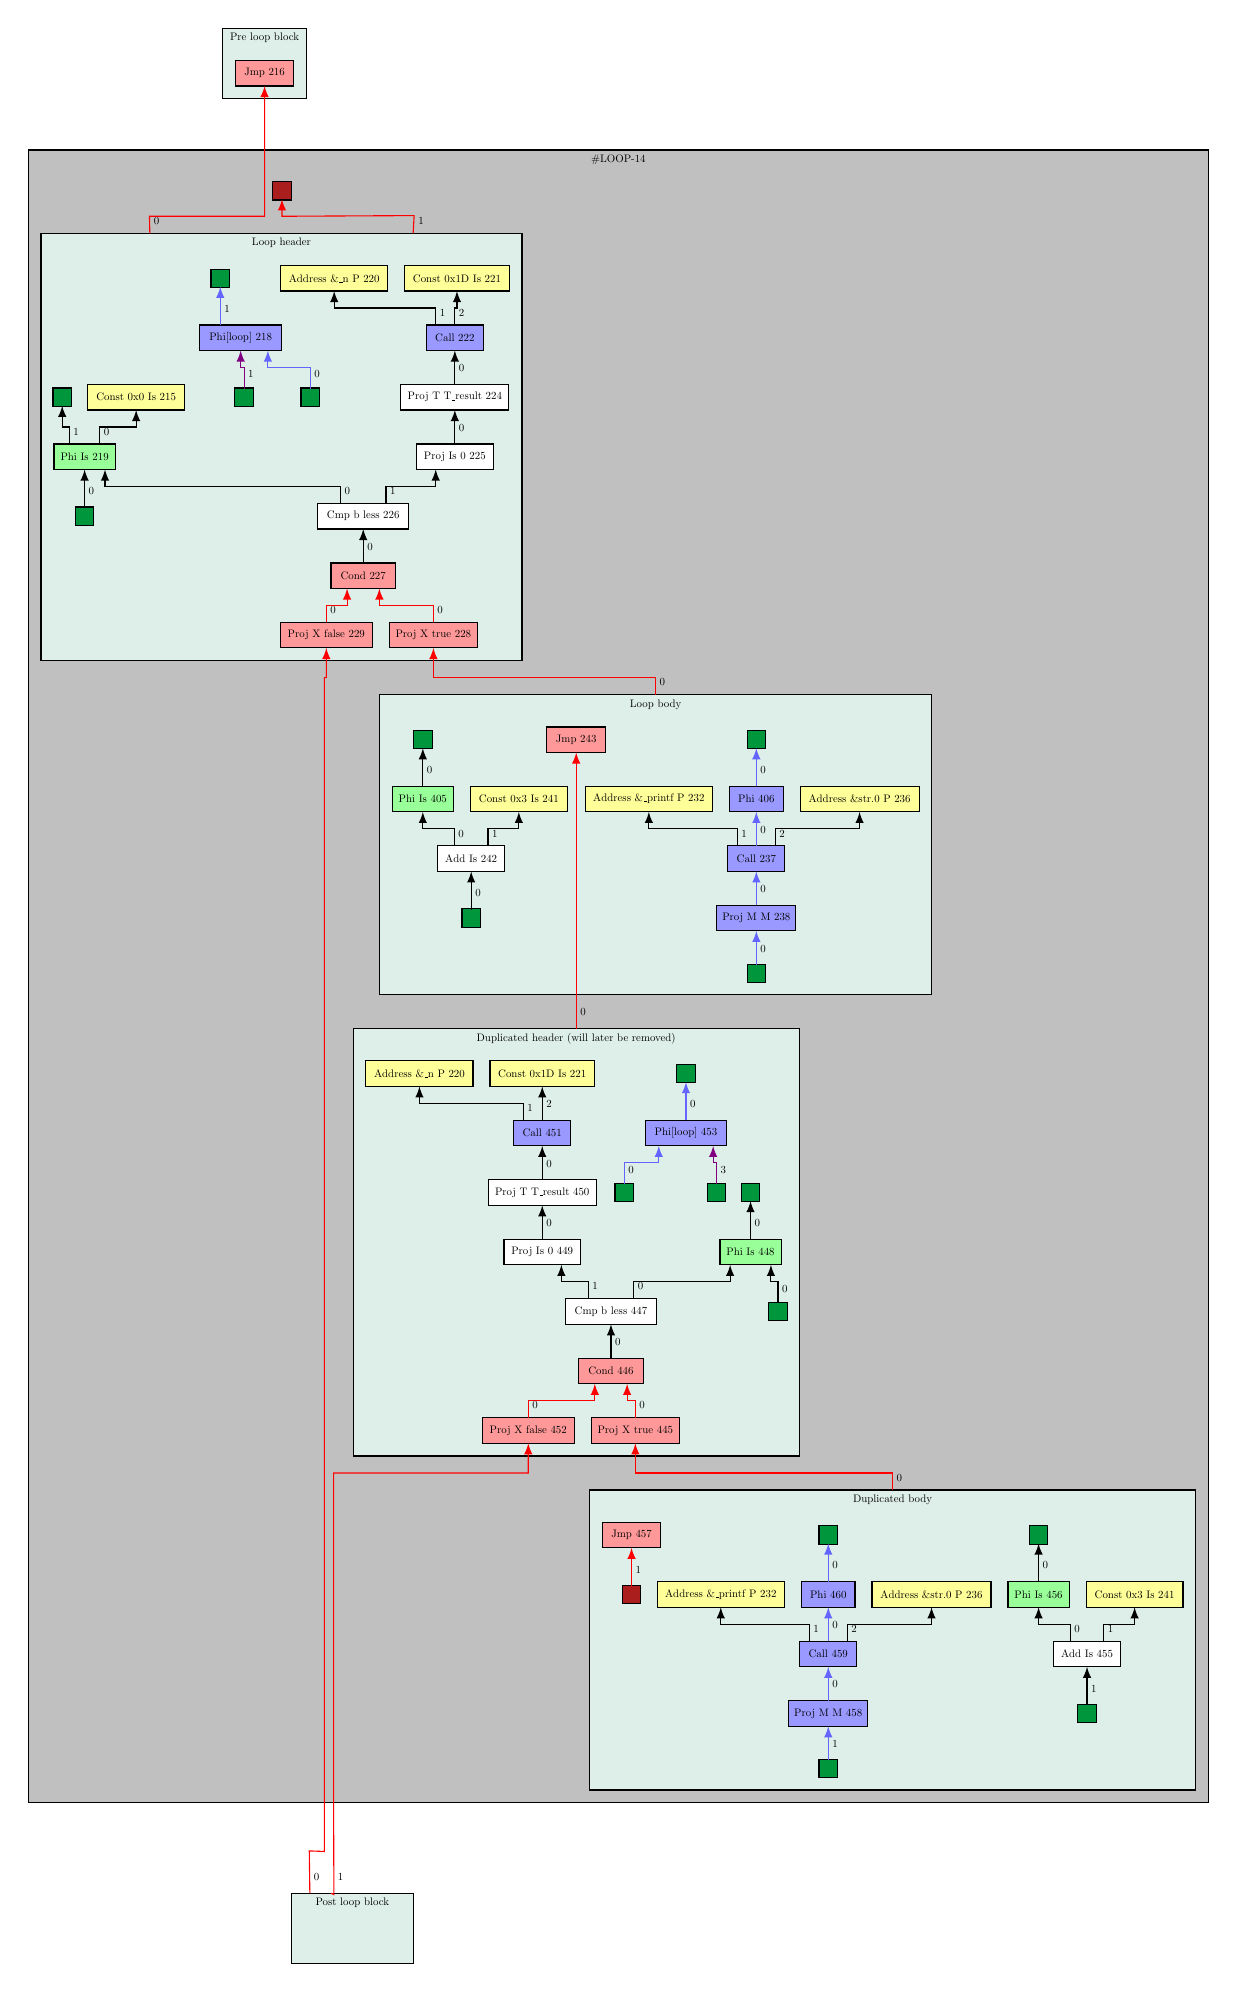
\begin{tikzpicture}
	\node[fill=color33, draw, minimum width=1.0683453237410072cm, minimum height=0.8956834532374102cm] (n101) at (11.222505742415636cm ,22.552094823164907cm) {};
	\node[fill=color34, draw, minimum width=14.989502857940924cm, minimum height=20.989208633093526cm] (n107) at (15.71598787432375cm ,10.958633093525181cm) {};
	% 1 node layouts
	\node[scale=0.3924133420536298, transform shape] at (11.222505742415636cm ,22.87667890589872cm) {Pre loop block};
	\node[fill=color33, draw, minimum width=7.699640287769787cm, minimum height=3.809352517985612cm] (n102) at (19.199048655812195cm ,2.5305755395683454cm) {};
	% 1 node layouts
	\node[scale=0.3924133420536298, transform shape] at (19.199048655812195cm ,4.311994154676259cm) {Duplicated body};
	\node[fill=color33, draw, minimum width=6.108812949640288cm, minimum height=5.428057553956835cm] (n103) at (11.437513423770554cm ,17.681654676258994cm) {};
	% 1 node layouts
	\node[scale=0.3924133420536298, transform shape] at (11.437513423770554cm ,20.27242580935252cm) {Loop header};
	\node[fill=color33, draw, minimum width=7.014388489208634cm, minimum height=3.809352517985612cm] (n104) at (16.189541668100926cm ,12.631294964028777cm) {};
	% 1 node layouts
	\node[scale=0.3924133420536298, transform shape] at (16.189541668100926cm ,14.41271357913669cm) {Loop body};
	\node[fill=color33, draw, minimum width=5.664977109221715cm, minimum height=5.428057553956835cm] (n105) at (15.18054886234553cm ,7.580935251798562cm) {};
	% 1 node layouts
	\node[scale=0.3924133420536298, transform shape] at (15.18054886234553cm ,10.171706384892087cm) {Duplicated header (will later be removed)};
	\node[fill=color33, draw, minimum width=1.5539568345323742cm, minimum height=0.8956834532374102cm] (n106) at (12.337230215827338cm ,-1.1337679856115108cm) {};
	% 1 node layouts
	\node[scale=0.3924133420536298, transform shape] at (12.337230215827338cm ,-0.8091839028776979cm) {Post loop block};
	% 1 node layouts
	\node[scale=0.3924133420536298, transform shape] at (15.71598787432375cm ,21.32997976618705cm) {\#LOOP-14};
	\node[fill=color35, draw, minimum width=0.7446043165467626cm, minimum height=0.32374100719424465cm] (n108) at (11.222505742415636cm ,22.427994103740446cm) {};
	% 1 node layouts
	\node[scale=0.3924133420536298, transform shape] at (11.222505742415636cm ,22.427994103740446cm) {Jmp  216};
	\node[fill=color36, draw, minimum width=1.0359712230215827cm, minimum height=0.32374100719424465cm] (n109) at (16.57429068706757cm ,8.967625899280575cm) {};
	% 1 node layouts
	\node[scale=0.3924133420536298, transform shape] at (16.57429068706757cm ,8.967625899280575cm) {Phi[loop]  453};
	\node[fill=color35, draw, minimum width=1.1654676258992807cm, minimum height=0.32374100719424465cm] (n110) at (14.571858541874635cm ,5.190647482014389cm) {};
	% 1 node layouts
	\node[scale=0.3924133420536298, transform shape] at (14.571858541874635cm ,5.190647482014389cm) {Proj X false 452};
	\node[fill=color35, draw, minimum width=1.1223021582733814cm, minimum height=0.32374100719424465cm] (n111) at (15.931570772090462cm ,5.190647482014389cm) {};
	% 1 node layouts
	\node[scale=0.3924133420536298, transform shape] at (15.931570772090462cm ,5.190647482014389cm) {Proj X true 445};
	\node[fill=color35, draw, minimum width=0.8201438848920863cm, minimum height=0.32374100719424465cm] (n112) at (15.62195255757117cm ,5.946043165467626cm) {};
	% 1 node layouts
	\node[scale=0.3924133420536298, transform shape] at (15.62195255757117cm ,5.946043165467626cm) {Cond  446};
	\node[fill=color37, draw, minimum width=1.154676258992806cm, minimum height=0.32374100719424465cm] (n113) at (15.62195255757117cm ,6.701438848920864cm) {};
	% 1 node layouts
	\node[scale=0.3924133420536298, transform shape] at (15.62195255757117cm ,6.701438848920864cm) {Cmp b less 447};
	\node[fill=color38, draw, minimum width=0.7769784172661871cm, minimum height=0.32374100719424465cm] (n114) at (17.394434571959657cm ,7.456834532374101cm) {};
	% 1 node layouts
	\node[scale=0.3924133420536298, transform shape] at (17.394434571959657cm ,7.456834532374101cm) {Phi Is 448};
	\node[fill=color37, draw, minimum width=0.9712230215827339cm, minimum height=0.32374100719424465cm] (n115) at (14.749139444425321cm ,7.456834532374101cm) {};
	% 1 node layouts
	\node[scale=0.3924133420536298, transform shape] at (14.749139444425321cm ,7.456834532374101cm) {Proj Is 0 449};
	\node[fill=color37, draw, minimum width=1.3705035971223023cm, minimum height=0.32374100719424465cm] (n116) at (14.749139444425321cm ,8.212230215827338cm) {};
	% 1 node layouts
	\node[scale=0.3924133420536298, transform shape] at (14.749139444425321cm ,8.212230215827338cm) {Proj T T\_result 450};
	\node[fill=color36, draw, minimum width=0.723021582733813cm, minimum height=0.32374100719424465cm] (n117) at (14.749139444425321cm ,8.967625899280575cm) {};
	% 1 node layouts
	\node[scale=0.3924133420536298, transform shape] at (14.749139444425321cm ,8.967625899280575cm) {Call  451};
	\node[fill=color39, draw, minimum width=1.3597122302158273cm, minimum height=0.32374100719424465cm] (n118) at (13.189786926439709cm ,9.723021582733814cm) {};
	% 1 node layouts
	\node[scale=0.3924133420536298, transform shape] at (13.189786926439709cm ,9.723021582733814cm) {Address \&\_n P 220};
	\node[fill=color39, draw, minimum width=1.3273381294964028cm, minimum height=0.32374100719424465cm] (n119) at (14.749139444425321cm ,9.723021582733814cm) {};
	% 1 node layouts
	\node[scale=0.3924133420536298, transform shape] at (14.749139444425321cm ,9.723021582733814cm) {Const 0x1D Is 221};
	\node[fill=color40, draw, minimum width=0.21582733812949642cm, minimum height=0.21582733812949642cm] (n120) at (15.79050635090014cm ,8.212230215827338cm) {};
	\node[fill=color40, draw, minimum width=0.21582733812949642cm, minimum height=0.21582733812949642cm] (n121) at (17.743253244294518cm ,6.701438848920864cm) {};
	\node[fill=color40, draw, minimum width=0.21582733812949642cm, minimum height=0.21582733812949642cm] (n122) at (16.57429068706757cm ,9.723021582733814cm) {};
	\node[fill=color40, draw, minimum width=0.21582733812949642cm, minimum height=0.21582733812949642cm] (n123) at (17.394434571959657cm ,8.212230215827338cm) {};
	\node[fill=color40, draw, minimum width=0.21582733812949642cm, minimum height=0.21582733812949642cm] (n124) at (16.962779895700667cm ,8.212230215827338cm) {};
	\node[fill=color36, draw, minimum width=1.0035971223021583cm, minimum height=0.32374100719424465cm] (n125) at (18.381602612646724cm ,1.5971223021582734cm) {};
	% 1 node layouts
	\node[scale=0.3924133420536298, transform shape] at (18.381602612646724cm ,1.5971223021582734cm) {Proj M M 458};
	\node[fill=color36, draw, minimum width=0.723021582733813cm, minimum height=0.32374100719424465cm] (n126) at (18.381602612646724cm ,2.352517985611511cm) {};
	% 1 node layouts
	\node[scale=0.3924133420536298, transform shape] at (18.381602612646724cm ,2.352517985611511cm) {Call  459};
	\node[fill=color39, draw, minimum width=1.6187050359712232cm, minimum height=0.32374100719424465cm] (n127) at (17.01649469897766cm ,3.1079136690647484cm) {};
	% 1 node layouts
	\node[scale=0.3924133420536298, transform shape] at (17.01649469897766cm ,3.1079136690647484cm) {Address \&\_printf P 232};
	\node[fill=color39, draw, minimum width=1.510791366906475cm, minimum height=0.32374100719424465cm] (n128) at (19.692753691783416cm ,3.1079136690647484cm) {};
	% 1 node layouts
	\node[scale=0.3924133420536298, transform shape] at (19.692753691783416cm ,3.1079136690647484cm) {Address \&str.0 P 236};
	\node[fill=color36, draw, minimum width=0.6798561151079137cm, minimum height=0.32374100719424465cm] (n129) at (18.381602612646724cm ,3.1079136690647484cm) {};
	% 1 node layouts
	\node[scale=0.3924133420536298, transform shape] at (18.381602612646724cm ,3.1079136690647484cm) {Phi  460};
	\node[fill=color35, draw, minimum width=0.7446043165467626cm, minimum height=0.32374100719424465cm] (n130) at (15.883401173797804cm ,3.863309352517986cm) {};
	% 1 node layouts
	\node[scale=0.3924133420536298, transform shape] at (15.883401173797804cm ,3.863309352517986cm) {Jmp  457};
	\node[fill=color37, draw, minimum width=0.8525179856115108cm, minimum height=0.32374100719424465cm] (n131) at (21.66795924162925cm ,2.352517985611511cm) {};
	% 1 node layouts
	\node[scale=0.3924133420536298, transform shape] at (21.66795924162925cm ,2.352517985611511cm) {Add Is 455};
	\node[fill=color39, draw, minimum width=1.2302158273381296cm, minimum height=0.32374100719424465cm] (n132) at (22.2718903824309cm ,3.1079136690647484cm) {};
	% 1 node layouts
	\node[scale=0.3924133420536298, transform shape] at (22.2718903824309cm ,3.1079136690647484cm) {Const 0x3 Is 241};
	\node[fill=color38, draw, minimum width=0.7769784172661871cm, minimum height=0.32374100719424465cm] (n133) at (21.052465921999243cm ,3.1079136690647484cm) {};
	% 1 node layouts
	\node[scale=0.3924133420536298, transform shape] at (21.052465921999243cm ,3.1079136690647484cm) {Phi Is 456};
	\node[fill=color40, draw, minimum width=0.21582733812949642cm, minimum height=0.21582733812949642cm] (n134) at (18.381602612646724cm ,3.863309352517986cm) {};
	\node[fill=color40, draw, minimum width=0.21582733812949642cm, minimum height=0.21582733812949642cm] (n135) at (21.052465921999243cm ,3.863309352517986cm) {};
	\node[fill=color40, draw, minimum width=0.21582733812949642cm, minimum height=0.21582733812949642cm] (n136) at (18.381602612646724cm ,0.8956834532374102cm) {};
	\node[fill=color40, draw, minimum width=0.21582733812949642cm, minimum height=0.21582733812949642cm] (n137) at (21.66795924162925cm ,1.5971223021582734cm) {};
	\node[fill=color36, draw, minimum width=1.0359712230215827cm, minimum height=0.32374100719424465cm] (n138) at (10.919078171971991cm ,19.06834532374101cm) {};
	% 1 node layouts
	\node[scale=0.3924133420536298, transform shape] at (10.919078171971991cm ,19.06834532374101cm) {Phi[loop]  218};
	\node[fill=color35, draw, minimum width=1.1654676258992807cm, minimum height=0.32374100719424465cm] (n139) at (12.006851703147051cm ,15.29136690647482cm) {};
	% 1 node layouts
	\node[scale=0.3924133420536298, transform shape] at (12.006851703147051cm ,15.29136690647482cm) {Proj X false 229};
	\node[fill=color35, draw, minimum width=1.1223021582733814cm, minimum height=0.32374100719424465cm] (n140) at (13.366563933362878cm ,15.29136690647482cm) {};
	% 1 node layouts
	\node[scale=0.3924133420536298, transform shape] at (13.366563933362878cm ,15.29136690647482cm) {Proj X true 228};
	\node[fill=color35, draw, minimum width=0.8201438848920863cm, minimum height=0.32374100719424465cm] (n141) at (12.475732848230985cm ,16.046762589928058cm) {};
	% 1 node layouts
	\node[scale=0.3924133420536298, transform shape] at (12.475732848230985cm ,16.046762589928058cm) {Cond  227};
	\node[fill=color37, draw, minimum width=1.154676258992806cm, minimum height=0.32374100719424465cm] (n142) at (12.475732848230985cm ,16.802158273381295cm) {};
	% 1 node layouts
	\node[scale=0.3924133420536298, transform shape] at (12.475732848230985cm ,16.802158273381295cm) {Cmp b less 226};
	\node[fill=color37, draw, minimum width=0.9712230215827339cm, minimum height=0.32374100719424465cm] (n143) at (13.63915835782331cm ,17.557553956834532cm) {};
	% 1 node layouts
	\node[scale=0.3924133420536298, transform shape] at (13.63915835782331cm ,17.557553956834532cm) {Proj Is 0 225};
	\node[fill=color37, draw, minimum width=1.3705035971223023cm, minimum height=0.32374100719424465cm] (n144) at (13.63915835782331cm ,18.31294964028777cm) {};
	% 1 node layouts
	\node[scale=0.3924133420536298, transform shape] at (13.63915835782331cm ,18.31294964028777cm) {Proj T T\_result 224};
	\node[fill=color36, draw, minimum width=0.723021582733813cm, minimum height=0.32374100719424465cm] (n145) at (13.63915835782331cm ,19.06834532374101cm) {};
	% 1 node layouts
	\node[scale=0.3924133420536298, transform shape] at (13.63915835782331cm ,19.06834532374101cm) {Call  222};
	\node[fill=color39, draw, minimum width=1.3597122302158273cm, minimum height=0.32374100719424465cm] (n146) at (12.10702781225976cm ,19.823741007194247cm) {};
	% 1 node layouts
	\node[scale=0.3924133420536298, transform shape] at (12.10702781225976cm ,19.823741007194247cm) {Address \&\_n P 220};
	\node[fill=color39, draw, minimum width=1.3273381294964028cm, minimum height=0.32374100719424465cm] (n147) at (13.666380330245373cm ,19.823741007194247cm) {};
	% 1 node layouts
	\node[scale=0.3924133420536298, transform shape] at (13.666380330245373cm ,19.823741007194247cm) {Const 0x1D Is 221};
	\node[fill=color38, draw, minimum width=0.7769784172661871cm, minimum height=0.32374100719424465cm] (n148) at (8.937157458542735cm ,17.557553956834532cm) {};
	% 1 node layouts
	\node[scale=0.3924133420536298, transform shape] at (8.937157458542735cm ,17.557553956834532cm) {Phi Is 219};
	\node[fill=color39, draw, minimum width=1.2302158273381296cm, minimum height=0.32374100719424465cm] (n149) at (9.591740042475589cm ,18.31294964028777cm) {};
	% 1 node layouts
	\node[scale=0.3924133420536298, transform shape] at (9.591740042475589cm ,18.31294964028777cm) {Const 0x0 Is 215};
	\node[fill=color40, draw, minimum width=0.21582733812949642cm, minimum height=0.21582733812949642cm] (n150) at (10.660085366216595cm ,19.823741007194247cm) {};
	\node[fill=color40, draw, minimum width=0.21582733812949642cm, minimum height=0.21582733812949642cm] (n151) at (8.65289112161228cm ,18.31294964028777cm) {};
	\node[fill=color40, draw, minimum width=0.21582733812949642cm, minimum height=0.21582733812949642cm] (n152) at (11.802902362619474cm ,18.31294964028777cm) {};
	\node[fill=color40, draw, minimum width=0.21582733812949642cm, minimum height=0.21582733812949642cm] (n153) at (8.937157458542735cm ,16.802158273381295cm) {};
	\node[fill=color40, draw, minimum width=0.21582733812949642cm, minimum height=0.21582733812949642cm] (n154) at (10.96224363959789cm ,18.31294964028777cm) {};
	\node[fill=color36, draw, minimum width=1.0035971223021583cm, minimum height=0.32374100719424465cm] (n155) at (17.468318646518192cm ,11.697841726618705cm) {};
	% 1 node layouts
	\node[scale=0.3924133420536298, transform shape] at (17.468318646518192cm ,11.697841726618705cm) {Proj M M 238};
	\node[fill=color36, draw, minimum width=0.723021582733813cm, minimum height=0.32374100719424465cm] (n156) at (17.468318646518192cm ,12.453237410071942cm) {};
	% 1 node layouts
	\node[scale=0.3924133420536298, transform shape] at (17.468318646518192cm ,12.453237410071942cm) {Call  237};
	\node[fill=color39, draw, minimum width=1.6187050359712232cm, minimum height=0.32374100719424465cm] (n157) at (16.103210732849128cm ,13.208633093525181cm) {};
	% 1 node layouts
	\node[scale=0.3924133420536298, transform shape] at (16.103210732849128cm ,13.208633093525181cm) {Address \&\_printf P 232};
	\node[fill=color39, draw, minimum width=1.510791366906475cm, minimum height=0.32374100719424465cm] (n158) at (18.77946972565488cm ,13.208633093525181cm) {};
	% 1 node layouts
	\node[scale=0.3924133420536298, transform shape] at (18.77946972565488cm ,13.208633093525181cm) {Address \&str.0 P 236};
	\node[fill=color36, draw, minimum width=0.6798561151079137cm, minimum height=0.32374100719424465cm] (n159) at (17.468318646518192cm ,13.208633093525181cm) {};
	% 1 node layouts
	\node[scale=0.3924133420536298, transform shape] at (17.468318646518192cm ,13.208633093525181cm) {Phi  406};
	\node[fill=color35, draw, minimum width=0.7446043165467626cm, minimum height=0.32374100719424465cm] (n160) at (15.18054886234553cm ,13.964028776978418cm) {};
	% 1 node layouts
	\node[scale=0.3924133420536298, transform shape] at (15.18054886234553cm ,13.964028776978418cm) {Jmp  243};
	\node[fill=color37, draw, minimum width=0.8525179856115108cm, minimum height=0.32374100719424465cm] (n161) at (13.84691576882035cm ,12.453237410071942cm) {};
	% 1 node layouts
	\node[scale=0.3924133420536298, transform shape] at (13.84691576882035cm ,12.453237410071942cm) {Add Is 242};
	\node[fill=color39, draw, minimum width=1.2302158273381296cm, minimum height=0.32374100719424465cm] (n162) at (14.452131596158479cm ,13.208633093525181cm) {};
	% 1 node layouts
	\node[scale=0.3924133420536298, transform shape] at (14.452131596158479cm ,13.208633093525181cm) {Const 0x3 Is 241};
	\node[fill=color38, draw, minimum width=0.7769784172661871cm, minimum height=0.32374100719424465cm] (n163) at (13.232707135726825cm ,13.208633093525181cm) {};
	% 1 node layouts
	\node[scale=0.3924133420536298, transform shape] at (13.232707135726825cm ,13.208633093525181cm) {Phi Is 405};
	\node[fill=color40, draw, minimum width=0.21582733812949642cm, minimum height=0.21582733812949642cm] (n164) at (17.468318646518192cm ,13.964028776978418cm) {};
	\node[fill=color40, draw, minimum width=0.21582733812949642cm, minimum height=0.21582733812949642cm] (n165) at (13.232707135726825cm ,13.964028776978418cm) {};
	\node[fill=color40, draw, minimum width=0.21582733812949642cm, minimum height=0.21582733812949642cm] (n166) at (17.468318646518192cm ,10.996402877697843cm) {};
	\node[fill=color40, draw, minimum width=0.21582733812949642cm, minimum height=0.21582733812949642cm] (n167) at (13.84691576882035cm ,11.697841726618705cm) {};
	\node[fill=color41, draw, minimum width=0.21582733812949642cm, minimum height=0.21582733812949642cm] (n168) at (11.44372876399837cm ,20.93525179856115cm) {};
	\node[fill=color41, draw, minimum width=0.21582733812949642cm, minimum height=0.21582733812949642cm] (n169) at (15.883401173797804cm ,3.1079136690647484cm) {};
	\draw[color=color42, -latex] (19.199048655812195cm ,4.4352517985611515cm) -- (19.19904865581219cm ,4.651079136690647cm) -- (15.931570772090462cm ,4.651079136690647cm) -- (15.931570772090462cm ,5.028776978417266cm);
	\node[] at (19.285379591063993cm ,4.592401079136691cm) {
		\scalebox{0.3924133420536298}{0}
	};
	\draw[color=color42, -latex] (9.7655494324636cm ,20.39568345323741cm) -- (9.760920011000769cm ,20.611510791366907cm) -- (11.222505742415636cm ,20.611510791366907cm) -- (11.222505742415636cm ,22.266123600143324cm);
	\node[] at (9.850608180996998cm ,20.552832733812952cm) {
		\scalebox{0.3924133420536298}{0}
	};
	\draw[color=color42, -latex] (16.189541668100926cm ,14.535971223021583cm) -- (16.189541668100926cm ,14.75179856115108cm) -- (13.366563933362878cm ,14.75179856115108cm) -- (13.366563933362878cm ,15.129496402877699cm);
	\node[] at (16.275872603352724cm ,14.693120503597124cm) {
		\scalebox{0.3924133420536298}{0}
	};
	\draw[color=color42, -latex] (15.18054886234553cm ,10.29496402877698cm) -- (15.18054886234553cm ,13.802158273381295cm);
	\node[] at (15.266879797597328cm ,10.502065535071942cm) {
		\scalebox{0.3924133420536298}{0}
	};
	\draw[color=color42, -latex] (11.797661870503598cm ,-0.6858714590827368cm) -- (11.790546954690896cm ,-0.14814226901732497cm) -- (11.981892086330935cm ,-0.15513669064747931cm) -- (11.981545385701008cm ,0.24820143884892087cm) -- (11.981545385701008cm ,14.75179856115108cm) -- (12.006851703147051cm ,14.75179856115108cm) -- (12.006851703147051cm ,15.129496402877699cm);
	\node[] at (11.88254783262315cm ,-0.47882475269784175cm) {
		\scalebox{0.3924133420536298}{0}
	};
	\draw[color=color42, -latex] (12.067446043165468cm ,-0.6858714590827368cm) -- (12.103153327338127cm ,-0.7027877697841727cm) -- (12.100250421672232cm ,0.14028776978417268cm) -- (12.100250421672232cm ,4.651079136690647cm) -- (14.571858541874635cm ,4.651079136690647cm) -- (14.571858541874635cm ,5.028776978417266cm);
	\node[] at (12.189049987902306cm ,-0.47882475269784175cm) {
		\scalebox{0.3924133420536298}{1}
	};
	\draw[color=color43, -latex] (16.57429068706757cm ,9.129496402877699cm) -- (16.57429068706757cm ,9.615107913669066cm);
	\node[] at (16.660621622319372cm ,9.336597909172662cm) {
		\scalebox{0.3924133420536298}{0}
	};
	\draw[color=color42, -latex] (14.571858541874635cm ,5.352517985611511cm) -- (14.571858541874635cm ,5.568345323741007cm) -- (15.416916586348147cm ,5.568345323741007cm) -- (15.416916586348147cm ,5.784172661870504cm);
	\node[] at (14.658189477126433cm ,5.5096672661870505cm) {
		\scalebox{0.3924133420536298}{0}
	};
	\draw[color=color42, -latex] (15.931570772090462cm ,5.352517985611511cm) -- (15.931570772090462cm ,5.568345323741007cm) -- (15.82698852879419cm ,5.568345323741007cm) -- (15.82698852879419cm ,5.784172661870504cm);
	\node[] at (16.01790170734226cm ,5.5096672661870505cm) {
		\scalebox{0.3924133420536298}{0}
	};
	\draw[color=color44, -latex] (15.62195255757117cm ,6.107913669064748cm) -- (15.62195255757117cm ,6.539568345323741cm);
	\node[] at (15.708283492822968cm ,6.315015175359712cm) {
		\scalebox{0.3924133420536298}{0}
	};
	\draw[color=color44, -latex] (15.91062162231937cm ,6.863309352517986cm) -- (15.91062162231937cm ,7.079136690647482cm) -- (17.135441766204263cm ,7.079136690647482cm) -- (17.135441766204263cm ,7.294964028776978cm);
	\node[] at (15.99695255757117cm ,7.020458633093526cm) {
		\scalebox{0.3924133420536298}{0}
	};
	\draw[color=color44, -latex] (15.333283492822968cm ,6.863309352517986cm) -- (15.333283492822968cm ,7.079136690647482cm) -- (14.991945199821004cm ,7.079136690647482cm) -- (14.991945199821004cm ,7.294964028776978cm);
	\node[] at (15.419614428074766cm ,7.020458633093526cm) {
		\scalebox{0.3924133420536298}{1}
	};
	\draw[color=color44, -latex] (17.394434571959657cm ,7.618705035971224cm) -- (17.394434571959657cm ,8.10431654676259cm);
	\node[] at (17.48076550721146cm ,7.8258065422661875cm) {
		\scalebox{0.3924133420536298}{0}
	};
	\draw[color=color44, -latex] (14.749139444425321cm ,7.618705035971224cm) -- (14.749139444425321cm ,8.050359712230216cm);
	\node[] at (14.835470379677119cm ,7.8258065422661875cm) {
		\scalebox{0.3924133420536298}{0}
	};
	\draw[color=color44, -latex] (14.749139444425321cm ,8.374100719424462cm) -- (14.749139444425321cm ,8.805755395683454cm);
	\node[] at (14.835470379677119cm ,8.581202225719425cm) {
		\scalebox{0.3924133420536298}{0}
	};
	\draw[color=color44, -latex] (14.508132250180717cm ,9.129496402877699cm) -- (14.508132250180717cm ,9.345323741007194cm) -- (13.189786926439709cm ,9.345323741007194cm) -- (13.189786926439709cm ,9.56115107913669cm);
	\node[] at (14.594463185432515cm ,9.286645683453237cm) {
		\scalebox{0.3924133420536298}{1}
	};
	\draw[color=color44, -latex] (14.749139444425321cm ,9.129496402877699cm) -- (14.749139444425321cm ,9.56115107913669cm);
	\node[] at (14.835470379677119cm ,9.336597909172662cm) {
		\scalebox{0.3924133420536298}{2}
	};
	\draw[color=color43, -latex] (15.79050635090014cm ,8.320143884892087cm) -- (15.79050635090014cm ,8.589928057553957cm) -- (16.22896694606038cm ,8.589928057553957cm) -- (16.22896694606038cm ,8.805755395683454cm);
	\node[] at (15.87683728615194cm ,8.504271582733814cm) {
		\scalebox{0.3924133420536298}{0}
	};
	\draw[color=color44, -latex] (17.743253244294518cm ,6.809352517985612cm) -- (17.743253244294518cm ,7.079136690647482cm) -- (17.653427377715055cm ,7.079136690647482cm) -- (17.653427377715055cm ,7.294964028776978cm);
	\node[] at (17.829584179546316cm ,6.993480215827338cm) {
		\scalebox{0.3924133420536298}{0}
	};
	\draw[color=color45, -latex] (16.962779895700667cm ,8.320143884892087cm) -- (16.962779895700667cm ,8.589928057553957cm) -- (16.919614428074766cm ,8.589928057553957cm) -- (16.919614428074766cm ,8.805755395683454cm);
	\node[] at (17.049110830952465cm ,8.504271582733814cm) {
		\scalebox{0.3924133420536298}{3}
	};
	\draw[color=color43, -latex] (18.381602612646724cm ,1.7589928057553958cm) -- (18.381602612646724cm ,2.1906474820143886cm);
	\node[] at (18.467933547898525cm ,1.9660943120503598cm) {
		\scalebox{0.3924133420536298}{0}
	};
	\draw[color=color43, -latex] (18.381602612646724cm ,2.514388489208633cm) -- (18.381602612646724cm ,2.9460431654676262cm);
	\node[] at (18.467933547898525cm ,2.7214899955035974cm) {
		\scalebox{0.3924133420536298}{0}
	};
	\draw[color=color44, -latex] (18.14059541840212cm ,2.514388489208633cm) -- (18.14059541840212cm ,2.73021582733813cm) -- (17.01649469897766cm ,2.73021582733813cm) -- (17.01649469897766cm ,2.9460431654676262cm);
	\node[] at (18.22692635365392cm ,2.6715377697841727cm) {
		\scalebox{0.3924133420536298}{1}
	};
	\draw[color=color44, -latex] (18.62260980689133cm ,2.514388489208633cm) -- (18.62260980689133cm ,2.73021582733813cm) -- (19.692753691783416cm ,2.73021582733813cm) -- (19.692753691783416cm ,2.9460431654676262cm);
	\node[] at (18.708940742143128cm ,2.6715377697841727cm) {
		\scalebox{0.3924133420536298}{2}
	};
	\draw[color=color43, -latex] (18.381602612646724cm ,3.2697841726618706cm) -- (18.381602612646724cm ,3.7553956834532376cm);
	\node[] at (18.467933547898525cm ,3.4768856789568345cm) {
		\scalebox{0.3924133420536298}{0}
	};
	\draw[color=color44, -latex] (21.454829745226377cm ,2.514388489208633cm) -- (21.454829745226377cm ,2.73021582733813cm) -- (21.052465921999243cm ,2.73021582733813cm) -- (21.052465921999243cm ,2.9460431654676262cm);
	\node[] at (21.541160680478175cm ,2.6715377697841727cm) {
		\scalebox{0.3924133420536298}{0}
	};
	\draw[color=color44, -latex] (21.88108873803213cm ,2.514388489208633cm) -- (21.88108873803213cm ,2.73021582733813cm) -- (22.2718903824309cm ,2.73021582733813cm) -- (22.2718903824309cm ,2.9460431654676262cm);
	\node[] at (21.967419673283928cm ,2.6715377697841727cm) {
		\scalebox{0.3924133420536298}{1}
	};
	\draw[color=color44, -latex] (21.052465921999243cm ,3.2697841726618706cm) -- (21.052465921999243cm ,3.7553956834532376cm);
	\node[] at (21.13879685725104cm ,3.4768856789568345cm) {
		\scalebox{0.3924133420536298}{0}
	};
	\draw[color=color43, -latex] (18.381602612646724cm ,1.0035971223021583cm) -- (18.381602612646724cm ,1.4352517985611513cm);
	\node[] at (18.467933547898525cm ,1.2106986285971224cm) {
		\scalebox{0.3924133420536298}{1}
	};
	\draw[color=color44, -latex] (21.66795924162925cm ,1.7050359712230216cm) -- (21.66795924162925cm ,2.1906474820143886cm);
	\node[] at (21.754290176881053cm ,1.9121374775179858cm) {
		\scalebox{0.3924133420536298}{1}
	};
	\draw[color=color43, -latex] (10.660085366216595cm ,19.23021582733813cm) -- (10.660085366216595cm ,19.715827338129497cm);
	\node[] at (10.746416301468393cm ,19.437317333633093cm) {
		\scalebox{0.3924133420536298}{1}
	};
	\draw[color=color42, -latex] (12.006851703147051cm ,15.453237410071944cm) -- (12.006851703147051cm ,15.66906474820144cm) -- (12.270696877007962cm ,15.66906474820144cm) -- (12.270696877007962cm ,15.884892086330936cm);
	\node[] at (12.093182638398849cm ,15.610386690647482cm) {
		\scalebox{0.3924133420536298}{0}
	};
	\draw[color=color42, -latex] (13.366563933362878cm ,15.453237410071944cm) -- (13.366563933362878cm ,15.66906474820144cm) -- (12.680768819454006cm ,15.66906474820144cm) -- (12.680768819454006cm ,15.884892086330936cm);
	\node[] at (13.452894868614676cm ,15.610386690647482cm) {
		\scalebox{0.3924133420536298}{0}
	};
	\draw[color=color44, -latex] (12.475732848230985cm ,16.20863309352518cm) -- (12.475732848230985cm ,16.640287769784173cm);
	\node[] at (12.562063783482783cm ,16.415734599820144cm) {
		\scalebox{0.3924133420536298}{0}
	};
	\draw[color=color44, -latex] (12.187063783482783cm ,16.964028776978417cm) -- (12.187063783482783cm ,17.179856115107913cm) -- (9.196150264298131cm ,17.179856115107913cm) -- (9.196150264298131cm ,17.39568345323741cm);
	\node[] at (12.27339471873458cm ,17.12117805755396cm) {
		\scalebox{0.3924133420536298}{0}
	};
	\draw[color=color44, -latex] (12.764401912979185cm ,16.964028776978417cm) -- (12.764401912979185cm ,17.179856115107913cm) -- (13.396352602427626cm ,17.179856115107913cm) -- (13.396352602427626cm ,17.39568345323741cm);
	\node[] at (12.850732848230985cm ,17.12117805755396cm) {
		\scalebox{0.3924133420536298}{1}
	};
	\draw[color=color44, -latex] (13.63915835782331cm ,17.719424460431657cm) -- (13.63915835782331cm ,18.151079136690647cm);
	\node[] at (13.725489293075109cm ,17.92652596672662cm) {
		\scalebox{0.3924133420536298}{0}
	};
	\draw[color=color44, -latex] (13.63915835782331cm ,18.474820143884894cm) -- (13.63915835782331cm ,18.906474820143885cm);
	\node[] at (13.725489293075109cm ,18.681921650179856cm) {
		\scalebox{0.3924133420536298}{0}
	};
	\draw[color=color44, -latex] (13.398151163578707cm ,19.23021582733813cm) -- (13.398151163578707cm ,19.44604316546763cm) -- (12.10702781225976cm ,19.44604316546763cm) -- (12.10702781225976cm ,19.66187050359712cm);
	\node[] at (13.484482098830506cm ,19.38736510791367cm) {
		\scalebox{0.3924133420536298}{1}
	};
	\draw[color=color44, -latex] (13.63915835782331cm ,19.23021582733813cm) -- (13.63915835782331cm ,19.44604316546763cm) -- (13.666380330245373cm ,19.44604316546763cm) -- (13.666380330245373cm ,19.66187050359712cm);
	\node[] at (13.725489293075109cm ,19.38736510791367cm) {
		\scalebox{0.3924133420536298}{2}
	};
	\draw[color=color44, -latex] (9.131402062859282cm ,17.719424460431657cm) -- (9.131402062859282cm ,17.93525179856115cm) -- (9.591740042475589cm ,17.93525179856115cm) -- (9.591740042475589cm ,18.151079136690647cm);
	\node[] at (9.21773299811108cm ,17.876573741007196cm) {
		\scalebox{0.3924133420536298}{0}
	};
	\draw[color=color44, -latex] (8.742912854226187cm ,17.719424460431657cm) -- (8.742912854226187cm ,17.93525179856115cm) -- (8.65289112161228cm ,17.93525179856115cm) -- (8.65289112161228cm ,18.205035971223023cm);
	\node[] at (8.829243789477987cm ,17.876573741007196cm) {
		\scalebox{0.3924133420536298}{1}
	};
	\draw[color=color43, -latex] (11.802902362619474cm ,18.42086330935252cm) -- (11.802902362619474cm ,18.690647482014388cm) -- (11.264401912979185cm ,18.690647482014388cm) -- (11.264401912979185cm ,18.906474820143885cm);
	\node[] at (11.889233297871273cm ,18.604991007194247cm) {
		\scalebox{0.3924133420536298}{0}
	};
	\draw[color=color44, -latex] (8.937157458542735cm ,16.910071942446045cm) -- (8.937157458542735cm ,17.39568345323741cm);
	\node[] at (9.023488393794533cm ,17.117173448741006cm) {
		\scalebox{0.3924133420536298}{0}
	};
	\draw[color=color45, -latex] (10.96224363959789cm ,18.42086330935252cm) -- (10.96224363959789cm ,18.690647482014388cm) -- (10.919078171971991cm ,18.690647482014388cm) -- (10.919078171971991cm ,18.906474820143885cm);
	\node[] at (11.048574574849688cm ,18.604991007194247cm) {
		\scalebox{0.3924133420536298}{1}
	};
	\draw[color=color43, -latex] (17.468318646518192cm ,11.859712230215829cm) -- (17.468318646518192cm ,12.29136690647482cm);
	\node[] at (17.55464958176999cm ,12.066813736510792cm) {
		\scalebox{0.3924133420536298}{0}
	};
	\draw[color=color43, -latex] (17.468318646518192cm ,12.615107913669066cm) -- (17.468318646518192cm ,13.046762589928058cm);
	\node[] at (17.55464958176999cm ,12.822209419964029cm) {
		\scalebox{0.3924133420536298}{0}
	};
	\draw[color=color44, -latex] (17.22731145227359cm ,12.615107913669066cm) -- (17.22731145227359cm ,12.830935251798563cm) -- (16.103210732849128cm ,12.830935251798563cm) -- (16.103210732849128cm ,13.046762589928058cm);
	\node[] at (17.313642387525388cm ,12.772257194244604cm) {
		\scalebox{0.3924133420536298}{1}
	};
	\draw[color=color44, -latex] (17.709325840762794cm ,12.615107913669066cm) -- (17.709325840762794cm ,12.830935251798563cm) -- (18.77946972565488cm ,12.830935251798563cm) -- (18.77946972565488cm ,13.046762589928058cm);
	\node[] at (17.795656776014592cm ,12.772257194244604cm) {
		\scalebox{0.3924133420536298}{2}
	};
	\draw[color=color43, -latex] (17.468318646518192cm ,13.370503597122303cm) -- (17.468318646518192cm ,13.85611510791367cm);
	\node[] at (17.55464958176999cm ,13.577605103417266cm) {
		\scalebox{0.3924133420536298}{0}
	};
	\draw[color=color44, -latex] (13.633786272417472cm ,12.615107913669066cm) -- (13.633786272417472cm ,12.830935251798563cm) -- (13.232707135726825cm ,12.830935251798563cm) -- (13.232707135726825cm ,13.046762589928058cm);
	\node[] at (13.720117207669272cm ,12.772257194244604cm) {
		\scalebox{0.3924133420536298}{0}
	};
	\draw[color=color44, -latex] (14.060045265223229cm ,12.615107913669066cm) -- (14.060045265223229cm ,12.830935251798563cm) -- (14.452131596158479cm ,12.830935251798563cm) -- (14.452131596158479cm ,13.046762589928058cm);
	\node[] at (14.146376200475027cm ,12.772257194244604cm) {
		\scalebox{0.3924133420536298}{1}
	};
	\draw[color=color44, -latex] (13.232707135726825cm ,13.370503597122303cm) -- (13.232707135726825cm ,13.85611510791367cm);
	\node[] at (13.319038070978623cm ,13.577605103417266cm) {
		\scalebox{0.3924133420536298}{0}
	};
	\draw[color=color43, -latex] (17.468318646518192cm ,11.10431654676259cm) -- (17.468318646518192cm ,11.535971223021583cm);
	\node[] at (17.55464958176999cm ,11.311418053057555cm) {
		\scalebox{0.3924133420536298}{0}
	};
	\draw[color=color44, -latex] (13.84691576882035cm ,11.805755395683454cm) -- (13.84691576882035cm ,12.29136690647482cm);
	\node[] at (13.933246704072149cm ,12.012856901978418cm) {
		\scalebox{0.3924133420536298}{0}
	};
	\draw[color=color42, -latex] (13.109477415077507cm ,20.39568345323741cm) -- (13.122114180665038cm ,20.620143884892087cm) -- (11.44372876399837cm ,20.611510791366907cm) -- (11.44372876399837cm ,20.827338129496404cm);
	\node[] at (13.210406795310364cm ,20.55714928057554cm) {
		\scalebox{0.3924133420536298}{1}
	};
	\draw[color=color42, -latex] (15.883401173797804cm ,3.2158273381294964cm) -- (15.883401173797804cm ,3.7014388489208634cm);
	\node[] at (15.969732109049604cm ,3.4229288444244608cm) {
		\scalebox{0.3924133420536298}{1}
	};
\end{tikzpicture}

    \end{adjustbox}
    \caption{Firm graph of the loop shown in \cref{fig:impl:unroll:unroll-factor-2-before} unrolled with a factor of two}
    \label{fig:impl:unroll:unroll-factor-2-after}
\end{figure}

\newpage

\section{Fixup strategies}\label{sec:impl:fixup}

In \cref{sec:impl:unroll} we discussed the unrolling process.
There, we did not consider the fixup code needed, but instead plainly focused on unrolling the loop.
Firstly, we will now focus on making the loop run less than or equal times compared to the original loop in section~\cref{sec:impl:fixup:header-cond}.
Less-than or equal is not good enough though, we want our transformed loop to run exactly as often as the original loop.
Therefore, we will create fixup code, as discussed in this section.
\Cref{sec:impl:fixup:duff} uses a generalized version of Duff's device to create the required fixup code, whereas in \cref{sec:impl:fixup:loop} a copy of the original loop will be used.
After that, in \cref{sec:eval}, we evaluate, which approach yields faster binary run-times.

To see the reason why and to understand what is required of fixup code, we formally lay out conditions that need to be met in the equations~(\ref{eqn:impl:fixup:duff:conserve-semantics-identity}) through~(\ref{eqn:impl:fixup:duff:fixup-i-mult}).

Let $M \in \mathbb{N}_0$ be the number of times a loop runs before the transformation; $\Mloop \in \mathbb{N}_0$, $\Mfixup \in \mathbb{N}_0$ the number of times the unrolled body will run in the unrolled loop, or the fixup code respectively, after the transformation.
Further, the unroll-factor will be again denoted by $f \in \mathbb{N}, f > 1$.
Henceforth, we will assume all arithmetic operations to be integer operations for integers in the interval $\lbrack t_{min}, t_{max} \rbrack$.
Please note that integer division will be assumed to round towards zero: For example $\frac{5}{3} \overset{\text{integer divison}}{=} 1$.
Another convention we will introduce is that any interval will be integral, meaning it will only contain integers.
Additionally $x \mp y$ is henceforth defined as
$\begin{cases}
     x + y &, x < 0\\
     x - y &, x > 0
\end{cases}$

We will now lay out properties that form the basis of further arithmetic considerations.
The primary identity that is to be conserved, to retain the original semantics, is shown below in \cref{eqn:impl:fixup:duff:conserve-semantics-identity}.
Since we know our original loop ran $M$ times, we know that our transformed loop and the fixup code must in total also run $M$ times.

\begin{equation}\label{eqn:impl:fixup:duff:conserve-semantics-identity}
\begin{aligned}
    M = \Mloop + \Mfixup
\end{aligned}
\end{equation}

In order to use Duff's device, we need to restrict the amount of times the fixup code needs to run.
With the kept semantics in mind, we will maximize $\Mloop$ and minimize $\Mfixup$.

\begin{equation}\label{eqn:impl:fixup:duff:loop-iterations}
\begin{aligned}
    \Mloop &\overset{\text{integer divison}}{=} \frac{M}{f} \cdot f\\
    &\overset{\text{integer divison}}{\in} \medspace \rbrack M-f,M \rbrack
\end{aligned}
\end{equation}
By construction of the unrolled loop, \cref{eqn:impl:fixup:duff:loop-iterations} is always true, as the unrolled loop tries to run as often as possible, while running less than or equal times to the original loop.
\begin{proof}\label{proof:impl:fixup:duff:loop-iterations}
To prove the conjecture of \cref{eqn:impl:fixup:duff:loop-iterations}, consider the assumption
\[\Mloop = M - f - b,  b \in \left \lbrack 0, f \right\lbrack \]
and hence
\[\Mloop \leq M - f \Rightarrow \Mloop \notin \medspace \rbrack M-f,f \rbrack,\]
then by rerunning the unrolled again the body would be executed $f$ times causing $\Mloop = M - b \in \medspace \rbrack M-f,f \rbrack$, which would be a contradiction of the assumption.
We then induct this pattern for $\Mloop = M - nf - b, n \in \mathbb{N}_{+}, b \in \lbrack 0, f \lbrack $.
In these cases, the loop must merely be iterated multiple times.
\end{proof}

As the loop runs as often as possible, the fixup code will always run less times than the unroll factor.

\begin{equation}\label{eqn:impl:fixup:duff:fixup-interval}
\begin{aligned}
    \Mfixup \in \lbrack0, f\lbrack
\end{aligned}
\end{equation}

\begin{proof}\label{proof:impl:fixup:duff:fixup-interval}
Conjecture: $\Mfixup \in \lbrack0, f\lbrack$.\\

Assume $\Mfixup = f' > (f - 1)$
\begin{align*}
    \Mloop + \Mfixup &\overset{\ref{eqn:impl:fixup:duff:loop-iterations}}{\geq} M - (f - 1) + f' \\
    &> M - (f - 1) + (f - 1) \\
    &= M \medspace \overset{\ref{eqn:impl:fixup:duff:conserve-semantics-identity}}{\mLightning}
\end{align*}
\end{proof}

For the following mathematical considerations, we need to round up in integer division.
The following lemma describes how this can be accomplished.
\begin{lem}\label{lem:impl:fixup:duff:ceil-mp}
    Given $Y \neq 0: \medspace \ceil{\frac{X}{Y}} = \frac{X + (Y \mp 1)}{Y}$
\end{lem}

\begin{proof}
    To prove \cref{lem:impl:fixup:duff:ceil-mp}, we will consider cases $X \mod Y = 0$ and $X \mod Y \neq 0$.
    Further, we will assume $Y > 0$, since the proof for $Y < 0$ can be performed analogously.
    Consider the case that $X \mod Y = 0$.
    In this case $\exists n \in \mathbb{N}: n \cdot Y = X$ and $\ceil{\frac{X}{Y}} = \frac{X}{Y} = n~(\star)$.
    \begin{align*}
        \Rightarrow \frac{X + (Y - 1)}{Y} &= \frac{n \cdot Y + (Y - 1)}{Y}\\
        &=\underbrace{\frac{(n + 1) \cdot Y - 1}{Y}}_{< \frac{(n + 1) \cdot Y}{Y}}\\
        &\overset{\text{integer divison}}{=} \frac{n \cdot Y}{Y}\\
        &= n\\
        &\overset{\star}{=} \ceil{\frac{X}{Y}}
    \end{align*}
    Now consider $X \mod Y \neq 0$.
    In this case $\exists n \in \mathbb{N}: n \cdot Y < X < (n + 1) \cdot Y~(\star)$ and $\ceil{\frac{X}{Y}} \overset{\text{integer division}}{=} n + 1$.
    \begin{align*}
        \Rightarrow n \cdot Y + (Y - 1) < X + (Y - 1) < (n + 1) \cdot Y + (Y - 1)\\
        \Rightarrow (n + 1) \cdot Y \overset{\star}{\leq} X + (Y - 1) < (n + 2) \cdot Y\\
        \overset{Y > 0}{\Rightarrow} \frac{(n + 1) \cdot Y}{Y} \leq \frac{X + (Y - 1)}{Y} < \frac{(n + 2) \cdot Y}{Y}
    \end{align*}
    \begin{align*}
        \Rightarrow \frac{X + (Y - 1)}{Y} &\overset{\text{integer divison}}= n + 1\\
        &= \ceil{\frac{X}{Y}}
    \end{align*}
\end{proof}

Using our now derived lemma, we use the loop parameters $I$, $N$ and $c$ to calculate the total number of loop iterations.

\begin{equation}\label{eqn:impl:fixup:duff:total-iteration-based-on-bounds}
\begin{aligned}
    M &= \ceil{\frac{N - I}{c}} \\
    & \overset{\text{integer divison}}{=} \frac{N - I + (c \mp 1)}{c}
\end{aligned}
\end{equation}

With this result we can then in the actual product calculate $M$ accurately, since it is generally unknown.
Since $I$ is not the initial value for the fixup's counter, we will need to calculate it based on known parameters.

\begin{equation}\label{eqn:impl:fixup:duff:i-after-loop}
\begin{aligned}
    \ipl = c \cdot \Mloop + I
\end{aligned}
\end{equation}

We can then use the last two equations to calculate $\Mfixup$ based on only quantities that are known at either compile-time or at run-time.

\begin{equation}\label{eqn:impl:fixup:duff:fixup-i}
\begin{aligned}
    \Mfixup & \overset{\ref{eqn:impl:fixup:duff:conserve-semantics-identity}}{=} M - \Mloop \\
    & \overset{\ref{eqn:impl:fixup:duff:total-iteration-based-on-bounds}}{=}
    \frac{N - I + (c \mp 1)}{c} - \Mloop \\
    & \overset{\ref{eqn:impl:fixup:duff:i-after-loop}}{=}
    \frac{N - I + (c \mp 1)}{c} - \frac{\ipl + I}{c} \\
    &= \frac{N - I + I - \ipl + (c \mp 1)}{c}\\
    &= \frac{N - \ipl + (c \mp 1)}{c}
\end{aligned}
\end{equation}

As the above equation has a costly divison operation in it, we will rearrange it, such that it never needs to be computed at runtime.

\begin{equation}\label{eqn:impl:fixup:duff:fixup-i-mult}
\begin{aligned}
    (\ref{eqn:impl:fixup:duff:fixup-i}) &\overset{\text{integer division}}{\Longleftrightarrow} \Mfixup \cdot c = N - \ipl + (c \mp 1) \overset{\ref{eqn:impl:fixup:duff:fixup-interval}}{\in} \cinterval
\end{aligned}
\end{equation}

\Cref{eqn:impl:fixup:duff:fixup-i-mult} is especially significant in the construction of the generalization of Duff's device, as seen in~\cref{sec:impl:fixup:duff}.

\subsection{Updating the loop condition}\label{sec:impl:fixup:header-cond}

In the following sections~\ref{sec:impl:fixup:duff}, and~\ref{sec:impl:fixup:loop} we will use that $\Mloop = \frac{M}{f} \cdot f$.
Though, when unrolling (as described in~\cref{sec:impl:unroll}), the original bound ($N$) is kept.
Unfortunately, this does not guarantee $\Mloop$ to be correct, as made clear by an example where a loop with $I = 0, N = 3, c = 1, f = 2, cmp = <$ is unrolled.
In this example, this would yield the following: $\Mloop = 4 > M = 3 \mLightning$, due to the fact that after the first iteration of the unrolled loop $i = 2 < 3 = N$.
To combat this, we set the bound of the unrolled loop to $\hat{N} = N - c \cdot (f - 1)$.\footnote{N.B.: $c \cdot (f - 1)$ does not overflow, as per preconditions}
Now we will prove the conjecture that using the bound $\hat{N}$, the unrolled loop runs $\Mloop$ times, given the operation to calculate $\hat{N}$ will not over- or underflow.
\begin{proof}
    Let $\Mloop'$ be the number of times then unrolled loop with bound $\hat{N}$ runs.
    The proof is complete, iff $\Mloop' = \Mloop$.
    \begin{align*}
        \Mloop' &\overset{\text{loop construction}}{=} \ceil{\frac{\hat{N} - I}{c \cdot f}} \cdot f\\
        &\overset{\text{integer division}}{=} \frac{\hat{N} - I + (c \cdot f \mp 1)}{c \cdot f} \cdot f\\
        &= \frac{N - c \cdot (f - 1) - I + (c \cdot f \mp 1)}{c \cdot f} \cdot f\\
        &= \frac{N - c \cdot f + c - I + c \cdot f \mp 1}{c \cdot f} \cdot f\\
        &= \frac{N - I + c \mp 1}{c \cdot f} \cdot f\\
        &= \frac{\frac{N - I + c \mp 1}{c}}{f} \cdot f\\
        &\overset{\text{integer division}}{=} \frac{\ceil{\frac{N - I}{c}}}{f} \cdot f\\
        &\overset{\ref{eqn:impl:fixup:duff:total-iteration-based-on-bounds}}{=} \frac{M}{f} \cdot f\\
        &\overset{\ref{eqn:impl:fixup:duff:loop-iterations}}{=} \Mloop
    \end{align*}
\end{proof}

Therefore we change the header condition of the unrolled loop to $i~`cmp`~\hat{N}$.
Note that even though, we are calculating the rounding to a multiple of $f$ without the need for a slow divison operation.

\Cref{fig:impl:fixup:header-cond:firm} shows the comparison of the original condition to the changed header condition, for the loop shown in \cref{fig:impl:fixup:fixup-firm-loop}.
It is to be noted that the graph in graph with bound $\hat{N}$ can be constant folded to the same size, as the original header.

\begin{figure}[H]
	\begin{algorithmic}
		\State $i \gets 0$
		\While{i < 29}
			\State \Call{Print}{$\text{HelloWorld}$}
			\State $i \gets i + 3$
		\EndWhile
	\end{algorithmic}
	\caption{An example loop, for which the unrolling process will be explained}\label{fig:impl:fixup:fixup-firm-loop}
\end{figure}

\begin{figure}[H]
    \centering
    % Scale factor 0.06838709677419355
\definecolor{color10}{RGB}{255,255,255}
\definecolor{color11}{RGB}{153,255,153}
\definecolor{color12}{RGB}{255,255,153}
\definecolor{color13}{RGB}{0,150,60}
\definecolor{color14}{RGB}{0,0,0}
% Bounding Box: 409.0, 310.0
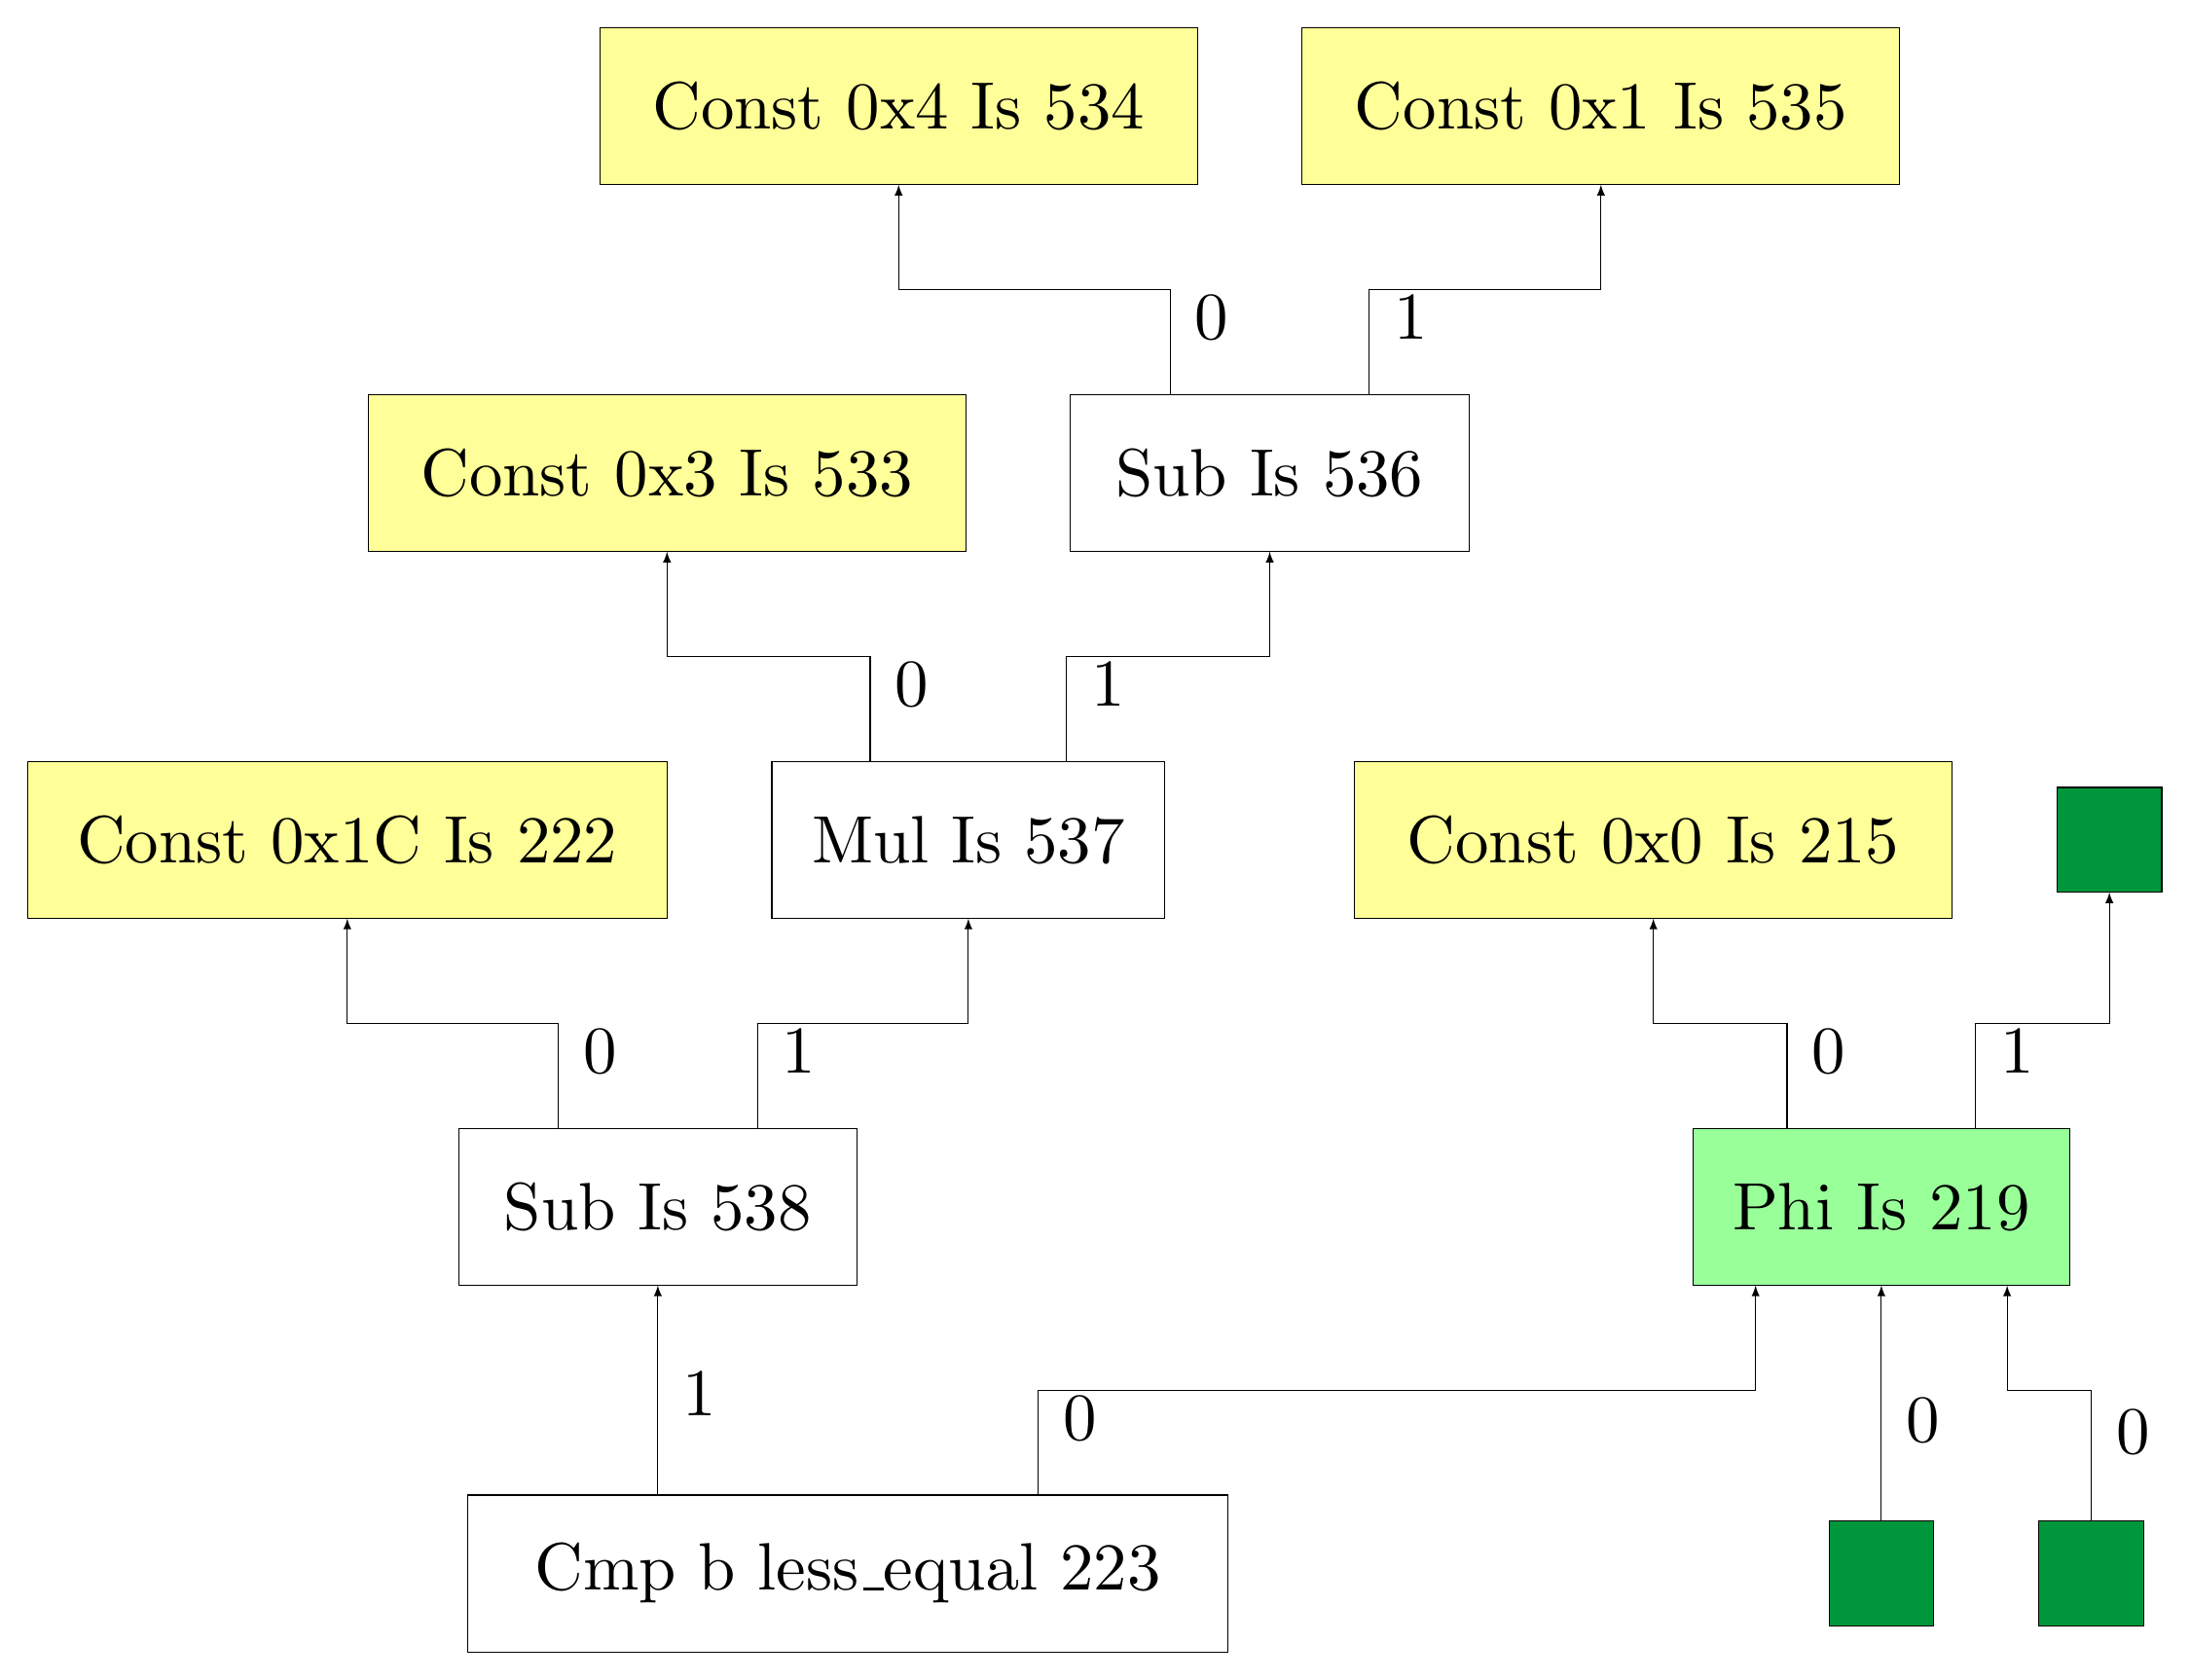
\begin{tikzpicture}
	\node[fill=color10, draw, minimum width=9.916129032258064cm, minimum height=2.0516129032258066cm] (n44) at (113.58092041890683cm ,-28.175483870967742cm) {};
	% 1 node layouts
	\node[scale=2.4868035190615836, transform shape] at (113.58092041890683cm ,-28.175483870967742cm) {Cmp b less\_equal 223};
	\node[fill=color11, draw, minimum width=4.9238709677419354cm, minimum height=2.0516129032258066cm] (n45) at (127.06635724686382cm ,-23.388387096774196cm) {};
	% 1 node layouts
	\node[scale=2.4868035190615836, transform shape] at (127.06635724686382cm ,-23.388387096774196cm) {Phi Is 219};
	\node[fill=color12, draw, minimum width=7.796129032258065cm, minimum height=2.0516129032258066cm] (n46) at (124.09151853718639cm ,-18.601290322580645cm) {};
	% 1 node layouts
	\node[scale=2.4868035190615836, transform shape] at (124.09151853718639cm ,-18.601290322580645cm) {Const 0x0 Is 215};
	\node[fill=color10, draw, minimum width=5.1974193548387095cm, minimum height=2.0516129032258066cm] (n47) at (111.10188816084231cm ,-23.388387096774196cm) {};
	% 1 node layouts
	\node[scale=2.4868035190615836, transform shape] at (111.10188816084231cm ,-23.388387096774196cm) {Sub Is 538};
	\node[fill=color12, draw, minimum width=8.343225806451613cm, minimum height=2.0516129032258066cm] (n48) at (107.04995267697134cm ,-18.601290322580645cm) {};
	% 1 node layouts
	\node[scale=2.4868035190615836, transform shape] at (107.04995267697134cm ,-18.601290322580645cm) {Const 0x1C Is 222};
	\node[fill=color10, draw, minimum width=5.129032258064516cm, minimum height=2.0516129032258066cm] (n49) at (115.15382364471328cm ,-18.601290322580645cm) {};
	% 1 node layouts
	\node[scale=2.4868035190615836, transform shape] at (115.15382364471328cm ,-18.601290322580645cm) {Mul Is 537};
	\node[fill=color12, draw, minimum width=7.796129032258065cm, minimum height=2.0516129032258066cm] (n50) at (111.22156558019715cm ,-13.814193548387097cm) {};
	% 1 node layouts
	\node[scale=2.4868035190615836, transform shape] at (111.22156558019715cm ,-13.814193548387097cm) {Const 0x3 Is 533};
	\node[fill=color10, draw, minimum width=5.1974193548387095cm, minimum height=2.0516129032258066cm] (n51) at (119.0860817092294cm ,-13.814193548387097cm) {};
	% 1 node layouts
	\node[scale=2.4868035190615836, transform shape] at (119.0860817092294cm ,-13.814193548387097cm) {Sub Is 536};
	\node[fill=color12, draw, minimum width=7.796129032258065cm, minimum height=2.0516129032258066cm] (n52) at (114.24377660170252cm ,-9.027096774193549cm) {};
	% 1 node layouts
	\node[scale=2.4868035190615836, transform shape] at (114.24377660170252cm ,-9.027096774193549cm) {Const 0x4 Is 534};
	\node[fill=color12, draw, minimum width=7.796129032258065cm, minimum height=2.0516129032258066cm] (n53) at (123.40764756944445cm ,-9.027096774193549cm) {};
	% 1 node layouts
	\node[scale=2.4868035190615836, transform shape] at (123.40764756944445cm ,-9.027096774193549cm) {Const 0x1 Is 535};
	\node[fill=color13, draw, minimum width=1.367741935483871cm, minimum height=1.367741935483871cm] (n54) at (129.80184111783154cm ,-28.175483870967742cm) {};
	\node[fill=color13, draw, minimum width=1.367741935483871cm, minimum height=1.367741935483871cm] (n55) at (130.04119595654123cm ,-18.601290322580645cm) {};
	\node[fill=color13, draw, minimum width=1.367741935483871cm, minimum height=1.367741935483871cm] (n56) at (127.06635724686382cm ,-28.175483870967742cm) {};
	\draw[color=color14, -latex] (116.05995267697135cm ,-27.14967741935484cm) -- (116.05995267697135cm ,-25.781935483870967cm) -- (125.42506692428317cm ,-25.781935483870967cm) -- (125.42506692428317cm ,-24.414193548387097cm);
	\node[] at (116.6070494511649cm ,-26.153790322580647cm) {
		\scalebox{2.4868035190615836}{0}
	};
	\draw[color=color14, -latex] (111.10188816084231cm ,-27.14967741935484cm) -- (111.10188816084231cm ,-24.414193548387097cm);
	\node[] at (111.64898493503586cm ,-25.837232862903228cm) {
		\scalebox{2.4868035190615836}{1}
	};
	\draw[color=color14, -latex] (125.83538950492833cm ,-22.36258064516129cm) -- (125.83538950492833cm ,-20.99483870967742cm) -- (124.09151853718639cm ,-20.99483870967742cm) -- (124.09151853718639cm ,-19.62709677419355cm);
	\node[] at (126.38248627912188cm ,-21.366693548387097cm) {
		\scalebox{2.4868035190615836}{0}
	};
	\draw[color=color14, -latex] (128.2973249887993cm ,-22.36258064516129cm) -- (128.2973249887993cm ,-20.99483870967742cm) -- (130.04119595654123cm ,-20.99483870967742cm) -- (130.04119595654123cm ,-19.28516129032258cm);
	\node[] at (128.84442176299285cm ,-21.366693548387097cm) {
		\scalebox{2.4868035190615836}{1}
	};
	\draw[color=color14, -latex] (109.80253332213263cm ,-22.36258064516129cm) -- (109.80253332213263cm ,-20.99483870967742cm) -- (107.04995267697134cm ,-20.99483870967742cm) -- (107.04995267697134cm ,-19.62709677419355cm);
	\node[] at (110.34963009632618cm ,-21.366693548387097cm) {
		\scalebox{2.4868035190615836}{0}
	};
	\draw[color=color14, -latex] (112.40124299955198cm ,-22.36258064516129cm) -- (112.40124299955198cm ,-20.99483870967742cm) -- (115.15382364471328cm ,-20.99483870967742cm) -- (115.15382364471328cm ,-19.62709677419355cm);
	\node[] at (112.94833977374553cm ,-21.366693548387097cm) {
		\scalebox{2.4868035190615836}{1}
	};
	\draw[color=color14, -latex] (113.87156558019714cm ,-17.575483870967744cm) -- (113.87156558019714cm ,-16.20774193548387cm) -- (111.22156558019715cm ,-16.20774193548387cm) -- (111.22156558019715cm ,-14.84cm);
	\node[] at (114.41866235439069cm ,-16.57959677419355cm) {
		\scalebox{2.4868035190615836}{0}
	};
	\draw[color=color14, -latex] (116.43608170922941cm ,-17.575483870967744cm) -- (116.43608170922941cm ,-16.20774193548387cm) -- (119.0860817092294cm ,-16.20774193548387cm) -- (119.0860817092294cm ,-14.84cm);
	\node[] at (116.98317848342296cm ,-16.57959677419355cm) {
		\scalebox{2.4868035190615836}{1}
	};
	\draw[color=color14, -latex] (117.78672687051973cm ,-12.788387096774194cm) -- (117.78672687051973cm ,-11.420645161290324cm) -- (114.24377660170252cm ,-11.420645161290324cm) -- (114.24377660170252cm ,-10.052903225806451cm);
	\node[] at (118.33382364471328cm ,-11.7925cm) {
		\scalebox{2.4868035190615836}{0}
	};
	\draw[color=color14, -latex] (120.38543654793908cm ,-12.788387096774194cm) -- (120.38543654793908cm ,-11.420645161290324cm) -- (123.40764756944445cm ,-11.420645161290324cm) -- (123.40764756944445cm ,-10.052903225806451cm);
	\node[] at (120.93253332213263cm ,-11.7925cm) {
		\scalebox{2.4868035190615836}{1}
	};
	\draw[color=color14, -latex] (129.80184111783154cm ,-27.491612903225807cm) -- (129.80184111783154cm ,-25.781935483870967cm) -- (128.70764756944445cm ,-25.781935483870967cm) -- (128.70764756944445cm ,-24.414193548387097cm);
	\node[] at (130.3489378920251cm ,-26.32475806451613cm) {
		\scalebox{2.4868035190615836}{0}
	};
	\draw[color=color14, -latex] (127.06635724686382cm ,-27.491612903225807cm) -- (127.06635724686382cm ,-24.414193548387097cm);
	\node[] at (127.61345402105736cm ,-26.179168346774194cm) {
		\scalebox{2.4868035190615836}{0}
	};
\end{tikzpicture}

    \caption{The changed header condition for \cref{fig:impl:fixup:duff:fixup-firm-loop} after constant folding}
    \label{fig:impl:fixup:header-cond:firm}
\end{figure}

We know that $c \cdot (f + 1)$ cannot over- or underflow, as per the preconditions laid out in \cref{sec:impl:unrollability}.
Since $f > 0$, $c \cdot (f - 1)$ will therefore also not overflow.
Though, $N - c \cdot (f - 1)$ can still over- or underflow, due to the subtraction of $c \cdot (f - 1)$ from $N$, and hence there is nevertheless a possibility to construct an example where this change does not conserve semantics.

Suppose the datatype of a loop with parameters $N = 2, I = 0, c = 1, cmp = <$ is an unsigned integer (with more than two bits), and we unroll this loop by a factor of four.
In this case $\hat{N} = 2 - 1 \cdot (4 - 1) = -1 \overset{\text{unsigned integer}}{=} t_{max}$.
With this bound the loop would run $t_{max} > 2$ times.

To circumvent this problem, we use \cref{alg:basics:overflow:detect} from \cref{sec:basics:overflow} as a check for over- or underflows of the operation.
We implement this check by placing a block between the header and its predecessors.
If an under- or overflow is detected, the control flow will jump directly the fixup code.
Otherwise, it will route the control flow to the header and let the loop progress as normal, given that $\hat{N}$ now restores semantics in the header.
\Cref{alg:impl:fixup:header-cond:preheader} shows the creation of this structure in~\libFIRM.

\begin{algorithm}[H]
    \begin{algorithmic}
        \Function{CreatePreHeader}{$header, firstFixupBlock: \text{block}, loop: \text{loop}$}
            \State $pre \gets\text{ }$ \Call{NewEmptyBlock}{}
            \State $pre.predecessors \gets \{node \vert node \in header.predecessors, node \notin loop\}$
            \For{$phi \in header.phis$}
                \State $phi' \gets\text{ }$ \Call{NewPhiInBlock}{$pre$}
                \State $phi'.predecessors \gets \{node \vert node \in phi.predecessors, node.block \notin loop\}$
                \State $phi.predecessors \gets \{phi'\} \cup \{node \vert node \in phi.predecessors, node.block \in loop\}$
                \For{$succ \in phi.successors$}
                    \If{$succ.block$~dominated by~$firstFixupBlock$}
                        \State $succ.predecessors$.prepend($pre$)
                    \EndIf
                \EndFor
            \EndFor
            \State $(trueExit, falseExit) \gets\text{ }$\Call{CreateOverflowCondition}{} \Comment{See \Cref{sec:basics:overflow}}
            \State $firstFixupBlock.predecessors.prepend(falseExit)$
            \State $header.predecessors \gets \{trueExit\} \cup \{node \vert node \in header.predecessors \cap loop\}$
        \EndFunction
    \end{algorithmic}
    \caption{Algorithm that creates the check to ensure $\hat{N}$ does not over- or underflow}
    \label{alg:impl:fixup:header-cond:preheader}
\end{algorithm}

\newpage

\subsection{Generalized Duff's device}\label{sec:impl:fixup:duff}

\Cref{sec:basics:duffs} describes the original version of Duff's device.
The problem with this initial approach is that it assumes $c = 1$, even though \hyperref[sec:impl::def-c]{$c$ is defined} as any non-zero integer in the considered loops.
Therefore, a need for generalization arises.

Using equations~\ref{eqn:impl:fixup:duff:conserve-semantics-identity} through~\ref{eqn:impl:fixup:duff:fixup-i-mult} and the general idea of Duff's device (see \cref{sec:basics:duffs}), we will create fixup code in form of a generalized Duff's device.
The structure of this fixup code can be seen in \cref{fig:impl:fixup:duff:fixup-M_fixup}, which we then practically implement, using \cref{eqn:impl:fixup:duff:fixup-i-mult}, as shown in \cref{fig:impl:fixup:duff:fixup-bound}.

\begin{figure}[H]
    \begin{algorithmic}
        \Switch{$\Mfixup$}
            \Case{$f - 1$}
                \State \Call{Body}{} \Comment{Fall-through}
            \EndCase
            \Case{$f - 2$}
                \State \Call{Body}{} \Comment{Fall-through}
            \EndCase
            \State \ldots
            \Case{$1$}
                \State \Call{Body}{}
            \EndCase
        \EndSwitch
    \end{algorithmic}
    \caption{Generalized Duff's device fixup code based on $\Mfixup$}
    \label{fig:impl:fixup:duff:fixup-M_fixup}
\end{figure}

\begin{figure}[H]
    \begin{algorithmic}
        \Switch{$N - \ipl + (c - 1)$}
            \Case{$c \cdot f \upto c \cdot (f + 1)$} \Comment flip bounds for $c < 0$
                \State \Call{Body}{}
            \EndCase
            \Case{$c \cdot (f - 1) \upto c \cdot f$}
                \State \Call{Body}{}
            \EndCase
            \State \ldots
            \Case{$c \cdot 1 \upto c \cdot 2$}
                \State \Call{Body}{}
            \EndCase
        \EndSwitch
    \end{algorithmic}
    \caption{Generalized duff's device fixup code based on variables present}
    \label{fig:impl:fixup:duff:fixup-bound}
\end{figure}

For the fixup code to work correctly, it is to be ensured that $(f + 1) \cdot c$ does not overflow, as otherwise, the interval \cinterval could potentially be invalid, iff an integer over- or underflow occurs, meaning $
\begin{cases}
    c \cdot (f + 1) < 0 &, \medspace c > 0\\
    c \cdot (f + 1) > 0 &, \medspace c < 0
\end{cases}$.
To avoid these problems altogether, c is restricted to being a compile-time constant, such that for integers defined from $t_{min}$ to $t_{max}$, $c \in \lbrack \frac{t_{min}}{f + 1}, \frac{t_{max}}{f + 1} \rbrack$.
Using this restriction, it can be asserted that $c \cdot (f + 1) \in \lbrack t_{min}, t_{max} \rbrack$ and therefore does not overflow.
\Cref{alg:impl:fixup:duff:create-fixup} details how the mechanics described above are translated into \libFIRM.
At first, we duplicate the loop body $f - 1$ times and add keepalive edges to all duplicated nodes, to make sure they do not disappear through implicit premature optimizations.
Then we will create the \textit{fixup header}, meaning a block, with the calculation of $n \coloneqq N - i + (c \mp 1)$.
$f - 1$ newly created condition blocks will then use the calculated value by the header.
In the $i^{\text{th}}$ (counting starts at 0) condition block, it will be checked whether $n$ is in the interval spanned by $c \cdot (f - i)$ and  $c \cdot (f - i + 1)$.\footnote{Please note: $c$ being positive or not determines, which limit is the upper and which is the lower bound.}
After this, we will wire all duplicated blocks such that they are reachable by the conditions.
Further, upon false evaluation of a condition, the following condition is evaluated, except if it is the last condition, in which case the false target is the post loop block.
Additionally, except in the case of the first duplicated header, they are attached to the previous blocks as fallthrough.
Lastly, the last block of the fixup code now precedes the post loop block, and the false exit fo the last condition.
An example of the result for creating fixup code for a loop and for $f = 2$, as seen in \cref{fig:impl:fixup:fixup-firm-loop}, can be seen in \cref{fig:impl:fixup:duff:fixup-firm}.
Further, \cref{fig:impl:fixup:duff:fixup-firm-comp} shows the completed unroll process with the added generalized Duff's device, given $f = 2$.
Once this process is completed~\cref{fig:impl:fixup:duff:general-loop} shows the resulting structure in pseudo-code notation.

\begin{figure}[H]
    \centering
    \begin{algorithmic}
        \Function{Foo}{$I \in \mathbb{Z}, N \in \mathbb{Z}, c \in \mathbb{Z} \backslash \zeroset, cmp \in \{<, >, \leq, \geq\}$}
        \State $i \gets I$
        \If{$N > c \cdot (f - 1)$}
            \While{$i~`cmp`~ (N - c \cdot (f - 1))$}
                \State \Call{DoSomething}{} \Comment{$f$ times}
                \State $i \gets i + c$ \Comment{$f$ times}
            \EndWhile
        \EndIf
        \Switch{$N - i + (c \mp 1)$}
            \Case{$c \cdot f \upto c \cdot (f + 1)$} \Comment flip bounds for $c < 0$
                \State \Call{DoSomething}{}
                \State $i \gets i + c$
            \EndCase
            \Case{$c \cdot (f - 1) \upto c \cdot f$}
                \State \Call{DoSomething}{}
                \State $i \gets i + c$
            \EndCase
            \State
            \ldots
            \Case{$c \cdot 1 \upto c \cdot 2$}
                \State \Call{DoSomething}{}
                \State $i \gets i + c$
            \EndCase
        \EndSwitch
        \EndFunction
    \end{algorithmic}
    \caption{The general form of loop starting at $I$ and counting in increments of $c$ up to $N$ transformed by the created loop unrolling with generalized duff's device fixup}
    \label{fig:impl:fixup:duff:general-loop}
\end{figure}

\begin{algorithm}[H]
    \caption{Algorithm to build generalized Duff's device fixup for a given loop in \libFIRM}
    \label{alg:impl:fixup:duff:create-fixup}
    \begin{algorithmic}
        \Function{CreateFixupSwitch}{$loop: \text{Loop}, factor: \mathbb{N}_{>1}$}
            \For{$i \in \{0, .., (factor - 1)\}$}
                \State \Call{DuplicateBody}{$loop$}
            \EndFor
            \For{$node \in allCopiedNodes$}
                \If{$\neg$\Call{HasKeepalive}{$node.link$}}
                    \State \Call{AddKeepAlive}{$node$} \Comment{Prevent premature disappearance}
                \EndIf
            \EndFor
            \State $relation \gets header.cmp.relation$
            \State $inverseRelation \gets\text{ }$ \Call{GetInverseRelation}{$relation$}
            \State $duffHeader \gets NewEmptyBlock$
            \State $duffHeader.predecessors \gets \{loop.header\}$
            \State $val \gets duffHeader.addNode(N - i + (c
                \left\{\!\begin{aligned}
                   - &, \medspace c > 0\\
                   + &, \medspace c < 0
                \end{aligned}\right\} 1)
            )$
            \State $i \gets 0$
            \State $prevLast: \text{Block}$
            \State $prevCond: \text{Block}$
            \For{$body \in duplicatedLoopBodies$}
                \State $firstBlock \gets\text{ }$ \Call{GetFirstBlockInBody}{$body$}
                \State $condBlock \gets\text{ }$ \Call{NewEmptyBlock}{}
                \State $cond \gets val \medspace `relation` \medspace (factor - i) \medspace \wedge \medspace val \medspace `inverseRelation` \medspace (factor - i - 1)$
                \State $condBlock.addNode(cond)$
                \State $condBlock.predecessors \gets \begin{cases}\{duffHeader\} &, \medspace i = 0\\ \{prevCond.falseExit, \medspace prevLast\} &, \medspace i \neq 0\end{cases}$
                \State $firstBlock.predecessors \gets cond.trueExit$
                \State $prevLast \gets\text{ }$ \Call{GetLastBlockInBody}{$body$}
                \State $prevCond \gets cond$
                \For{$phi \in body.phis$}
                    \State $phi.predecessors \gets \begin{cases}\{phi.link.predecessors\} &, \medspace i = 0\\ \{phi.link.predecessors, \medspace prevLast.exitFor(phi)\} &, \medspace i \neq 0\end{cases}$
                \EndFor
                \State $i \gets i + 1$
            \EndFor
            \For{$node \in allCopiedNodes$}
                \If{$\neg$\Call{HasKeepalive}{$node.link$}}
                    \State \Call{RemoveKeepAlive}{$node$}
                \EndIf
            \EndFor
            \State $postLoopBlock.predecessors \gets \{prevCond.falseExit, \medspace prevLast\}$
            \State \Call{RewirePhis}{} \Comment{Wire just like for duplicated loop body phi's}
        \EndFunction
    \end{algorithmic}
\end{algorithm}

\begin{figure}[H]
	\begin{algorithmic}
		\State $i \gets 0$
		\If{$\neg$\Call{SubtractionWillLeaveBounds}{$29 - 6$}}
			\While{i < 23}
				\State \Call{Print}{$\text{HelloWorld}$}
				\State $i \gets i + 3$
				\State \Call{Print}{$\text{HelloWorld}$}
				\State $i \gets i + 3$
			\EndWhile
		\EndIf
		\Switch{31 - i}
			\Case{$\lbrack 3, 6 \lbrack$}
				\State \Call{Print}{$\text{HelloWorld}$}
				\State $i \gets i + 3$
			\EndCase
		\EndSwitch
	\end{algorithmic}
	\caption{An example loop, as seen in \Cref{fig:impl:fixup:fixup-firm-loop}, unrolled by a factor of two, and with generalized Duff's device fixup}\label{fig:impl:fixup:duff:fixup-firm-comp}
\end{figure}

\begin{figure}
	\begin{adjustbox}{max height=\textheight}
		% Scale factor 0.02717391304347826
\definecolor{color0}{RGB}{222,239,234}
\definecolor{color1}{RGB}{153,153,255}
\definecolor{color2}{RGB}{255,255,255}
\definecolor{color3}{RGB}{255,255,153}
\definecolor{color4}{RGB}{153,255,153}
\definecolor{color5}{RGB}{255,153,153}
\definecolor{color6}{RGB}{0,150,60}
\definecolor{color7}{RGB}{255,0,0}
\definecolor{color8}{RGB}{100,100,255}
\definecolor{color9}{RGB}{0,0,0}
% Bounding Box: 552.0, 1332.0
\begin{tikzpicture}
	\node[fill=color0, draw, minimum width=13.301630434782608cm, minimum height=9.592391304347826cm] (n1) at (8.75679347826087cm ,-29.36141304347826cm) {};
	% 1 node layouts
	\node[scale=0.9881422924901185, transform shape] at (8.75679347826087cm ,-24.875594429347824cm) {Duff header};
	\node[fill=color0, draw, minimum width=10.516304347826086cm, minimum height=9.864130434782608cm] (n2) at (5.665760869565217cm ,-40.17663043478261cm) {};
	% 1 node layouts
	\node[scale=0.9881422924901185, transform shape] at (5.665760869565217cm ,-35.55494225543478cm) {Condition block};
	\node[fill=color0, draw, minimum width=12.744565217391305cm, minimum height=7.690217391304348cm] (n3) at (8.994565217391305cm ,-50.04076086956522cm) {};
	% 1 node layouts
	\node[scale=0.9881422924901185, transform shape] at (8.994565217391305cm ,-46.50602921195652cm) {Body};
	\node[fill=color0, draw, minimum width=6.168478260869565cm, minimum height=5.788043478260869cm] (n4) at (8.179347826086955cm ,-57.86684782608695cm) {};
	% 1 node layouts
	\node[scale=0.9881422924901185, transform shape] at (8.179347826086955cm ,-55.283203125cm) {Post loop block};
	\node[fill=color1, draw, minimum width=1.7119565217391304cm, minimum height=0.8152173913043478cm] (n5) at (3.369565217391304cm ,-27.907608695652172cm) {};
	% 1 node layouts
	\node[scale=0.9881422924901185, transform shape] at (3.369565217391304cm ,-27.907608695652172cm) {Phi  420};
	\node[fill=color2, draw, minimum width=2.1467391304347827cm, minimum height=0.8152173913043478cm] (n6) at (11.888586956521738cm ,-31.71195652173913cm) {};
	% 1 node layouts
	\node[scale=0.9881422924901185, transform shape] at (11.888586956521738cm ,-31.71195652173913cm) {Add Is 425};
	\node[fill=color3, draw, minimum width=3.0978260869565215cm, minimum height=0.8152173913043478cm] (n7) at (13.451086956521738cm ,-29.809782608695652cm) {};
	% 1 node layouts
	\node[scale=0.9881422924901185, transform shape] at (13.451086956521738cm ,-29.809782608695652cm) {Const 0x2 Is 514};
	\node[fill=color2, draw, minimum width=2.0652173913043477cm, minimum height=0.8152173913043478cm] (n8) at (10.326086956521738cm ,-29.809782608695652cm) {};
	% 1 node layouts
	\node[scale=0.9881422924901185, transform shape] at (10.326086956521738cm ,-29.809782608695652cm) {Sub Is 423};
	\node[fill=color4, draw, minimum width=1.9565217391304348cm, minimum height=0.8152173913043478cm] (n9) at (7.96195652173913cm ,-27.907608695652172cm) {};
	% 1 node layouts
	\node[scale=0.9881422924901185, transform shape] at (7.96195652173913cm ,-27.907608695652172cm) {Phi Is 440};
	\node[fill=color4, draw, minimum width=1.9565217391304348cm, minimum height=0.8152173913043478cm] (n10) at (12.051630434782608cm ,-27.907608695652172cm) {};
	% 1 node layouts
	\node[scale=0.9881422924901185, transform shape] at (12.051630434782608cm ,-27.907608695652172cm) {Phi Is 441};
	\node[fill=color3, draw, minimum width=3.0978260869565215cm, minimum height=0.8152173913043478cm] (n11) at (10.869565217391305cm ,-26.005434782608695cm) {};
	% 1 node layouts
	\node[scale=0.9881422924901185, transform shape] at (10.869565217391305cm ,-26.005434782608695cm) {Const 0x0 Is 215};
	\node[fill=color5, draw, minimum width=1.875cm, minimum height=0.8152173913043478cm] (n12) at (5.665760869565217cm ,-26.005434782608695cm) {};
	% 1 node layouts
	\node[scale=0.9881422924901185, transform shape] at (5.665760869565217cm ,-26.005434782608695cm) {Jmp  426};
	\node[fill=color6, draw, minimum width=0.5434782608695652cm, minimum height=0.5434782608695652cm] (n13) at (2.8260869565217392cm ,-26.005434782608695cm) {};
	\node[fill=color6, draw, minimum width=0.5434782608695652cm, minimum height=0.5434782608695652cm] (n14) at (3.9130434782608696cm ,-26.005434782608695cm) {};
	\node[fill=color6, draw, minimum width=0.5434782608695652cm, minimum height=0.5434782608695652cm] (n15) at (7.418478260869565cm ,-26.005434782608695cm) {};
	\node[fill=color6, draw, minimum width=0.5434782608695652cm, minimum height=0.5434782608695652cm] (n16) at (8.505434782608695cm ,-26.005434782608695cm) {};
	\node[fill=color6, draw, minimum width=0.5434782608695652cm, minimum height=0.5434782608695652cm] (n17) at (13.233695652173912cm ,-26.005434782608695cm) {};
	\node[fill=color6, draw, minimum width=0.5434782608695652cm, minimum height=0.5434782608695652cm] (n18) at (11.345108695652174cm ,-33.47826086956522cm) {};
	\node[fill=color6, draw, minimum width=0.5434782608695652cm, minimum height=0.5434782608695652cm] (n19) at (12.432065217391305cm ,-33.47826086956522cm) {};
	\node[fill=color6, draw, minimum width=0.5434782608695652cm, minimum height=0.5434782608695652cm] (n20) at (2.8260869565217392cm ,-29.809782608695652cm) {};
	\node[fill=color6, draw, minimum width=0.5434782608695652cm, minimum height=0.5434782608695652cm] (n21) at (3.9130434782608696cm ,-29.809782608695652cm) {};
	\node[fill=color5, draw, minimum width=2.934782608695652cm, minimum height=0.8152173913043478cm] (n22) at (3.953804347826087cm ,-44.29347826086956cm) {};
	% 1 node layouts
	\node[scale=0.9881422924901185, transform shape] at (3.953804347826087cm ,-44.29347826086956cm) {Proj X false 437};
	\node[fill=color5, draw, minimum width=2.8260869565217392cm, minimum height=0.8152173913043478cm] (n23) at (7.377717391304348cm ,-44.29347826086956cm) {};
	% 1 node layouts
	\node[scale=0.9881422924901185, transform shape] at (7.377717391304348cm ,-44.29347826086956cm) {Proj X true 436};
	\node[fill=color5, draw, minimum width=2.0652173913043477cm, minimum height=0.8152173913043478cm] (n24) at (5.665760869565217cm ,-42.391304347826086cm) {};
	% 1 node layouts
	\node[scale=0.9881422924901185, transform shape] at (5.665760869565217cm ,-42.391304347826086cm) {Cond  435};
	\node[fill=color2, draw, minimum width=2.092391304347826cm, minimum height=0.8152173913043478cm] (n25) at (5.665760869565217cm ,-40.48913043478261cm) {};
	% 1 node layouts
	\node[scale=0.9881422924901185, transform shape] at (5.665760869565217cm ,-40.48913043478261cm) {And b 434};
	\node[fill=color2, draw, minimum width=3.4510869565217392cm, minimum height=0.8152173913043478cm] (n26) at (7.7853260869565215cm ,-38.58695652173913cm) {};
	% 1 node layouts
	\node[scale=0.9881422924901185, transform shape] at (7.7853260869565215cm ,-38.58695652173913cm) {Cmp b greater 516};
	\node[fill=color3, draw, minimum width=3.0978260869565215cm, minimum height=0.8152173913043478cm] (n27) at (8.967391304347826cm ,-36.68478260869565cm) {};
	% 1 node layouts
	\node[scale=0.9881422924901185, transform shape] at (8.967391304347826cm ,-36.68478260869565cm) {Const 0x2 Is 514};
	\node[fill=color2, draw, minimum width=3.9402173913043477cm, minimum height=0.8152173913043478cm] (n28) at (3.546195652173913cm ,-38.58695652173913cm) {};
	% 1 node layouts
	\node[scale=0.9881422924901185, transform shape] at (3.546195652173913cm ,-38.58695652173913cm) {Cmp b less\_equal 519};
	\node[fill=color3, draw, minimum width=3.0978260869565215cm, minimum height=0.8152173913043478cm] (n29) at (2.3641304347826084cm ,-36.68478260869565cm) {};
	% 1 node layouts
	\node[scale=0.9881422924901185, transform shape] at (2.3641304347826084cm ,-36.68478260869565cm) {Const 0x5 Is 518};
	\node[fill=color6, draw, minimum width=0.5434782608695652cm, minimum height=0.5434782608695652cm] (n30) at (6.603260869565217cm ,-36.68478260869565cm) {};
	\node[fill=color6, draw, minimum width=0.5434782608695652cm, minimum height=0.5434782608695652cm] (n31) at (4.728260869565217cm ,-36.68478260869565cm) {};
	\node[fill=color1, draw, minimum width=2.527173913043478cm, minimum height=0.8152173913043478cm] (n32) at (6.154891304347826cm ,-51.440217391304344cm) {};
	% 1 node layouts
	\node[scale=0.9881422924901185, transform shape] at (6.154891304347826cm ,-51.440217391304344cm) {Proj M M 413};
	\node[fill=color1, draw, minimum width=1.8206521739130435cm, minimum height=0.8152173913043478cm] (n33) at (6.154891304347826cm ,-49.53804347826087cm) {};
	% 1 node layouts
	\node[scale=0.9881422924901185, transform shape] at (6.154891304347826cm ,-49.53804347826087cm) {Call  414};
	\node[fill=color3, draw, minimum width=4.076086956521739cm, minimum height=0.8152173913043478cm] (n34) at (6.154891304347826cm ,-47.63586956521739cm) {};
	% 1 node layouts
	\node[scale=0.9881422924901185, transform shape] at (6.154891304347826cm ,-47.63586956521739cm) {Address \&\_printf P 232};
	\node[fill=color3, draw, minimum width=3.8043478260869565cm, minimum height=0.8152173913043478cm] (n35) at (10.638586956521738cm ,-47.63586956521739cm) {};
	% 1 node layouts
	\node[scale=0.9881422924901185, transform shape] at (10.638586956521738cm ,-47.63586956521739cm) {Address \&str.0 P 236};
	\node[fill=color5, draw, minimum width=1.875cm, minimum height=0.8152173913043478cm] (n36) at (14.021739130434781cm ,-47.63586956521739cm) {};
	% 1 node layouts
	\node[scale=0.9881422924901185, transform shape] at (14.021739130434781cm ,-47.63586956521739cm) {Jmp  418};
	\node[fill=color6, draw, minimum width=0.5434782608695652cm, minimum height=0.5434782608695652cm] (n37) at (3.3016304347826084cm ,-47.63586956521739cm) {};
	\node[fill=color6, draw, minimum width=0.5434782608695652cm, minimum height=0.5434782608695652cm] (n38) at (6.154891304347826cm ,-53.20652173913043cm) {};
	\node[fill=color5, draw, minimum width=2.282608695652174cm, minimum height=0.8152173913043478cm] (n39) at (7.832880434782607cm ,-59.94565217391304cm) {};
	% 1 node layouts
	\node[scale=0.9881422924901185, transform shape] at (7.832880434782607cm ,-59.94565217391304cm) {Return  245};
	\node[fill=color3, draw, minimum width=3.0978260869565215cm, minimum height=0.8152173913043478cm] (n40) at (9.307065217391303cm ,-58.04347826086956cm) {};
	% 1 node layouts
	\node[scale=0.9881422924901185, transform shape] at (9.307065217391303cm ,-58.04347826086956cm) {Const 0x0 Is 215};
	\node[fill=color1, draw, minimum width=1.7119565217391304cm, minimum height=0.8152173913043478cm] (n41) at (6.358695652173911cm ,-58.04347826086956cm) {};
	% 1 node layouts
	\node[scale=0.9881422924901185, transform shape] at (6.358695652173911cm ,-58.04347826086956cm) {Phi  404};
	\node[fill=color6, draw, minimum width=0.5434782608695652cm, minimum height=0.5434782608695652cm] (n42) at (6.902173913043477cm ,-56.27717391304348cm) {};
	\node[fill=color6, draw, minimum width=0.5434782608695652cm, minimum height=0.5434782608695652cm] (n43) at (5.815217391304346cm ,-56.27717391304348cm) {};
	\draw[color=color7, -latex] (5.665760869565217cm ,-35.244565217391305cm) -- (5.665760869565217cm ,-26.413043478260867cm);
	\node[] at (5.883152173913043cm ,-34.723059612771735cm) {
		\scalebox{0.9881422924901185}{0}
	};
	\draw[color=color7, -latex] (8.994565217391305cm ,-46.19565217391304cm) -- (8.994565217391305cm ,-45.65217391304348cm) -- (7.377717391304348cm ,-45.65217391304348cm) -- (7.377717391304348cm ,-44.701086956521735cm);
	\node[] at (9.21195652173913cm ,-45.79993206521739cm) {
		\scalebox{0.9881422924901185}{0}
	};
	\draw[color=color7, -latex] (6.637228260869564cm ,-54.97282608695652cm) -- (6.637228260869564cm ,-54.42934782608695cm) -- (2.3369565217391304cm ,-54.42934782608695cm) -- (2.3369565217391304cm ,-45.65217391304348cm) -- (3.953804347826087cm ,-45.65217391304348cm) -- (3.953804347826087cm ,-44.701086956521735cm);
	\node[] at (6.85461956521739cm ,-54.57710597826087cm) {
		\scalebox{0.9881422924901185}{0}
	};
	\draw[color=color7, -latex] (9.721467391304346cm ,-54.97282608695652cm) -- (9.721467391304346cm ,-54.42934782608695cm) -- (14.021739130434781cm ,-54.42934782608695cm) -- (14.021739130434781cm ,-48.04347826086956cm);
	\node[] at (9.938858695652172cm ,-54.57710597826087cm) {
		\scalebox{0.9881422924901185}{1}
	};
	\draw[color=color8, -latex] (2.9415760869565215cm ,-27.5cm) -- (2.9415760869565215cm ,-26.956521739130434cm) -- (2.8260869565217392cm ,-26.956521739130434cm) -- (2.8260869565217392cm ,-26.277173913043477cm);
	\node[] at (3.1589673913043477cm ,-27.104279891304348cm) {
		\scalebox{0.9881422924901185}{0}
	};
	\draw[color=color8, -latex] (3.797554347826087cm ,-27.5cm) -- (3.797554347826087cm ,-26.956521739130434cm) -- (3.9130434782608696cm ,-26.956521739130434cm) -- (3.9130434782608696cm ,-26.277173913043477cm);
	\node[] at (4.014945652173913cm ,-27.104279891304348cm) {
		\scalebox{0.9881422924901185}{1}
	};
	\draw[color=color9, -latex] (11.351902173913043cm ,-31.304347826086957cm) -- (11.351902173913043cm ,-30.76086956521739cm) -- (10.326086956521738cm ,-30.76086956521739cm) -- (10.326086956521738cm ,-30.217391304347824cm);
	\node[] at (11.56929347826087cm ,-30.908627717391305cm) {
		\scalebox{0.9881422924901185}{0}
	};
	\draw[color=color9, -latex] (12.425271739130434cm ,-31.304347826086957cm) -- (12.425271739130434cm ,-30.76086956521739cm) -- (13.451086956521738cm ,-30.76086956521739cm) -- (13.451086956521738cm ,-30.217391304347824cm);
	\node[] at (12.64266304347826cm ,-30.908627717391305cm) {
		\scalebox{0.9881422924901185}{1}
	};
	\draw[color=color9, -latex] (9.809782608695652cm ,-29.402173913043477cm) -- (9.809782608695652cm ,-28.858695652173914cm) -- (7.96195652173913cm ,-28.858695652173914cm) -- (7.96195652173913cm ,-28.315217391304348cm);
	\node[] at (10.027173913043478cm ,-29.006453804347824cm) {
		\scalebox{0.9881422924901185}{0}
	};
	\draw[color=color9, -latex] (10.842391304347826cm ,-29.402173913043477cm) -- (10.842391304347826cm ,-28.858695652173914cm) -- (12.051630434782608cm ,-28.858695652173914cm) -- (12.051630434782608cm ,-28.315217391304348cm);
	\node[] at (11.059782608695652cm ,-29.006453804347824cm) {
		\scalebox{0.9881422924901185}{1}
	};
	\draw[color=color9, -latex] (7.4728260869565215cm ,-27.5cm) -- (7.4728260869565215cm ,-26.956521739130434cm) -- (7.418478260869565cm ,-26.956521739130434cm) -- (7.418478260869565cm ,-26.277173913043477cm);
	\node[] at (7.690217391304348cm ,-27.104279891304348cm) {
		\scalebox{0.9881422924901185}{0}
	};
	\draw[color=color9, -latex] (8.451086956521738cm ,-27.5cm) -- (8.451086956521738cm ,-26.956521739130434cm) -- (8.505434782608695cm ,-26.956521739130434cm) -- (8.505434782608695cm ,-26.277173913043477cm);
	\node[] at (8.668478260869565cm ,-27.104279891304348cm) {
		\scalebox{0.9881422924901185}{1}
	};
	\draw[color=color9, -latex] (11.5625cm ,-27.5cm) -- (11.5625cm ,-26.956521739130434cm) -- (10.869565217391305cm ,-26.956521739130434cm) -- (10.869565217391305cm ,-26.413043478260867cm);
	\node[] at (11.779891304347826cm ,-27.104279891304348cm) {
		\scalebox{0.9881422924901185}{0}
	};
	\draw[color=color9, -latex] (12.540760869565217cm ,-27.5cm) -- (12.540760869565217cm ,-26.956521739130434cm) -- (13.233695652173912cm ,-26.956521739130434cm) -- (13.233695652173912cm ,-26.277173913043477cm);
	\node[] at (12.758152173913043cm ,-27.104279891304348cm) {
		\scalebox{0.9881422924901185}{1}
	};
	\draw[color=color9, -latex] (11.345108695652174cm ,-33.20652173913044cm) -- (11.351902173913043cm ,-32.119565217391305cm);
	\node[] at (11.567299220872963cm ,-32.68501613451087cm) {
		\scalebox{0.9881422924901185}{0}
	};
	\draw[color=color9, -latex] (12.432065217391305cm ,-33.20652173913044cm) -- (12.425271739130434cm ,-32.119565217391305cm);
	\node[] at (12.647736922554346cm ,-32.68501613451087cm) {
		\scalebox{0.9881422924901185}{0}
	};
	\draw[color=color8, -latex] (2.8260869565217392cm ,-29.538043478260867cm) -- (2.8260869565217392cm ,-28.858695652173914cm) -- (2.9415760869565215cm ,-28.858695652173914cm) -- (2.9415760869565215cm ,-28.315217391304348cm);
	\node[] at (3.043478260869565cm ,-29.07438858695652cm) {
		\scalebox{0.9881422924901185}{0}
	};
	\draw[color=color8, -latex] (3.9130434782608696cm ,-29.538043478260867cm) -- (3.9130434782608696cm ,-28.858695652173914cm) -- (3.797554347826087cm ,-28.858695652173914cm) -- (3.797554347826087cm ,-28.315217391304348cm);
	\node[] at (4.130434782608695cm ,-29.07438858695652cm) {
		\scalebox{0.9881422924901185}{0}
	};
	\draw[color=color7, -latex] (3.953804347826087cm ,-43.88586956521739cm) -- (3.953804347826087cm ,-43.34239130434783cm) -- (5.14945652173913cm ,-43.34239130434783cm) -- (5.14945652173913cm ,-42.79891304347826cm);
	\node[] at (4.171195652173913cm ,-43.490149456521735cm) {
		\scalebox{0.9881422924901185}{0}
	};
	\draw[color=color7, -latex] (7.377717391304348cm ,-43.88586956521739cm) -- (7.377717391304348cm ,-43.34239130434783cm) -- (6.182065217391304cm ,-43.34239130434783cm) -- (6.182065217391304cm ,-42.79891304347826cm);
	\node[] at (7.595108695652174cm ,-43.490149456521735cm) {
		\scalebox{0.9881422924901185}{0}
	};
	\draw[color=color9, -latex] (5.665760869565217cm ,-41.983695652173914cm) -- (5.665760869565217cm ,-40.89673913043478cm);
	\node[] at (5.883152173913043cm ,-41.462190047554344cm) {
		\scalebox{0.9881422924901185}{0}
	};
	\draw[color=color9, -latex] (6.188858695652174cm ,-40.08152173913043cm) -- (6.188858695652174cm ,-39.53804347826087cm) -- (7.7853260869565215cm ,-39.53804347826087cm) -- (7.7853260869565215cm ,-38.994565217391305cm);
	\node[] at (6.40625cm ,-39.68580163043478cm) {
		\scalebox{0.9881422924901185}{0}
	};
	\draw[color=color9, -latex] (5.142663043478261cm ,-40.08152173913043cm) -- (5.142663043478261cm ,-39.53804347826087cm) -- (3.546195652173913cm ,-39.53804347826087cm) -- (3.546195652173913cm ,-38.994565217391305cm);
	\node[] at (5.360054347826087cm ,-39.68580163043478cm) {
		\scalebox{0.9881422924901185}{1}
	};
	\draw[color=color9, -latex] (8.648097826086957cm ,-38.17934782608695cm) -- (8.648097826086957cm ,-37.63586956521739cm) -- (8.967391304347826cm ,-37.63586956521739cm) -- (8.967391304347826cm ,-37.09239130434783cm);
	\node[] at (8.865489130434783cm ,-37.783627717391305cm) {
		\scalebox{0.9881422924901185}{1}
	};
	\draw[color=color9, -latex] (6.922554347826087cm ,-38.17934782608695cm) -- (6.922554347826087cm ,-37.63586956521739cm) -- (6.603260869565217cm ,-37.63586956521739cm) -- (6.603260869565217cm ,-36.95652173913044cm);
	\node[] at (7.139945652173913cm ,-37.783627717391305cm) {
		\scalebox{0.9881422924901185}{0}
	};
	\draw[color=color9, -latex] (2.561141304347826cm ,-38.17934782608695cm) -- (2.561141304347826cm ,-37.63586956521739cm) -- (2.3641304347826084cm ,-37.63586956521739cm) -- (2.3641304347826084cm ,-37.09239130434783cm);
	\node[] at (2.778532608695652cm ,-37.783627717391305cm) {
		\scalebox{0.9881422924901185}{1}
	};
	\draw[color=color9, -latex] (4.53125cm ,-38.17934782608695cm) -- (4.53125cm ,-37.63586956521739cm) -- (4.728260869565217cm ,-37.63586956521739cm) -- (4.728260869565217cm ,-36.95652173913044cm);
	\node[] at (4.748641304347826cm ,-37.783627717391305cm) {
		\scalebox{0.9881422924901185}{0}
	};
	\draw[color=color8, -latex] (6.154891304347826cm ,-51.03260869565217cm) -- (6.154891304347826cm ,-49.94565217391304cm);
	\node[] at (6.372282608695652cm ,-50.51110309103261cm) {
		\scalebox{0.9881422924901185}{0}
	};
	\draw[color=color9, -latex] (6.154891304347826cm ,-49.130434782608695cm) -- (6.154891304347826cm ,-48.04347826086956cm);
	\node[] at (6.372282608695652cm ,-48.60892917798913cm) {
		\scalebox{0.9881422924901185}{1}
	};
	\draw[color=color9, -latex] (6.76177536231884cm ,-49.130434782608695cm) -- (6.76177536231884cm ,-48.58695652173913cm) -- (10.638586956521738cm ,-48.58695652173913cm) -- (10.638586956521738cm ,-48.04347826086956cm);
	\node[] at (6.979166666666666cm ,-48.73471467391304cm) {
		\scalebox{0.9881422924901185}{2}
	};
	\draw[color=color8, -latex] (5.5480072463768115cm ,-49.130434782608695cm) -- (5.548007246376811cm ,-48.58695652173913cm) -- (3.3016304347826084cm ,-48.58695652173913cm) -- (3.3016304347826084cm ,-47.90760869565217cm);
	\node[] at (5.765398550724638cm ,-48.73471467391304cm) {
		\scalebox{0.9881422924901185}{0}
	};
	\draw[color=color8, -latex] (6.154891304347826cm ,-52.93478260869565cm) -- (6.154891304347826cm ,-51.84782608695652cm);
	\node[] at (6.372282608695652cm ,-52.413277004076086cm) {
		\scalebox{0.9881422924901185}{1}
	};
	\draw[color=color8, -latex] (7.262228260869564cm ,-59.53804347826087cm) -- (7.262228260869564cm ,-58.994565217391305cm) -- (6.358695652173911cm ,-58.994565217391305cm) -- (6.358695652173911cm ,-58.451086956521735cm);
	\node[] at (7.47961956521739cm ,-59.14232336956522cm) {
		\scalebox{0.9881422924901185}{0}
	};
	\draw[color=color9, -latex] (8.40353260869565cm ,-59.53804347826087cm) -- (8.40353260869565cm ,-58.994565217391305cm) -- (9.307065217391303cm ,-58.994565217391305cm) -- (9.307065217391303cm ,-58.451086956521735cm);
	\node[] at (8.620923913043477cm ,-59.14232336956522cm) {
		\scalebox{0.9881422924901185}{1}
	};
	\draw[color=color8, -latex] (6.786684782608694cm ,-57.63586956521739cm) -- (6.786684782608694cm ,-57.09239130434783cm) -- (6.902173913043477cm ,-57.09239130434783cm) -- (6.902173913043477cm ,-56.54891304347826cm);
	\node[] at (7.00407608695652cm ,-57.240149456521735cm) {
		\scalebox{0.9881422924901185}{0}
	};
	\draw[color=color8, -latex] (5.930706521739129cm ,-57.63586956521739cm) -- (5.930706521739129cm ,-57.09239130434783cm) -- (5.815217391304346cm ,-57.09239130434783cm) -- (5.815217391304346cm ,-56.54891304347826cm);
	\node[] at (6.148097826086955cm ,-57.240149456521735cm) {
		\scalebox{0.9881422924901185}{1}
	};
\end{tikzpicture}

	\end{adjustbox}
	\caption{Fixup code for the loop from \Cref{fig:impl:fixup:fixup-firm-loop}, given $f = 2$ in \libFIRM}\label{fig:impl:fixup:duff:fixup-firm}
\end{figure}

\subsection{Loop duplication}\label{sec:impl:fixup:loop}

Another, perhaps simpler, way of creating fixup code is, to duplicate the original loop, such that it will run $\Mloop$ times after the unrolled loop.
Just like when using the generalized form of Duff's device, we unroll the loop using the existing mechanics by a factor of $f$.
Therefore, equations~\ref{eqn:impl:fixup:duff:conserve-semantics-identity} through~\ref{eqn:impl:fixup:duff:i-after-loop} still hold true.

The approach now taken is to copy the original loop, change its initial value to $\ipl$ and use it as fixup code, as seen in \cref{fig:impl:fixup:loop:fixup-loop}.

\begin{figure}[H]
    \begin{algorithmic}
        \State $i \gets \ipl$
        \While{$i~`cmp`~N$}
            \State \Call{Body}{}
            \State $i \gets i + c$
        \EndWhile
    \end{algorithmic}
    \caption{The loop to run the body the remaining $\Mfixup$ times}
    \label{fig:impl:fixup:loop:fixup-loop}
\end{figure}

\begin{proof}
    To prove that this fixup code preserves semantics, first note that $\Mloop \overset{\ref{eqn:impl:fixup:duff:loop-iterations}}{\leq} M$.
    Then consider two cases:
    \begin{enumerate}
        \item $\Mloop = M$
        \item $\Mloop < M$
    \end{enumerate}
    In the first case, $\ipl~`cmp`~N$ must be false, as otherwise the unrolled loop would have broken semantics, and hence the new loop is never run.
    Therefore: $\Mfixup = 0 \Rightarrow \Mloop + \Mfixup = M$

    In the second case, the new loop runs until the condition is met.
    As the unrolled loop kept the increment semantics intact, the result is hence $\Mfixup = M - \Mloop$, which conserves the semantics, as per \cref{eqn:impl:fixup:duff:conserve-semantics-identity}.
\end{proof}

\Cref{alg:impl:fixup:loop:fixup-loop} shows how we create this structure in~\libFIRM.
Firstly, we copy the loop, after which we rewire it, such that the fixup loop points to it, and its old successors point to the fixup loop.
Once this is completed, we can unroll the original loop.
\Cref{fig:impl:fixup:loop:general-loop} shows the resulting structure of the entire process in pseudo-code notation.

\Cref{fig:impl:fixup:loop:fixup-firm-comp} shows the result for unroll the loop from \cref{fig:impl:fixup:fixup-firm-loop} using loop duplication fixup code and a factor of two.

\begin{figure}[H]
	\begin{algorithmic}
		\State $i \gets 0$
		\If{$\neg$\Call{SubtractionWillLeaveBounds}{$29 - 6$}}
			\While{i < 23}
				\State \Call{Print}{$\text{HelloWorld}$}
				\State $i \gets i + 3$
				\State \Call{Print}{$\text{HelloWorld}$}
				\State $i \gets i + 3$
			\EndWhile
		\EndIf
		\While{i < 29}
			\State \Call{Print}{$\text{HelloWorld}$}
			\State $i \gets i + 3$
		\EndWhile
	\end{algorithmic}
	\caption{An example loop, as seen in \Cref{fig:impl:fixup:fixup-firm-loop}, unrolled by a factor of two, and with loop duplication fixup}\label{fig:impl:fixup:loop:fixup-firm-comp}
\end{figure}

\begin{figure}[H]
    \centering
    \begin{algorithmic}
        \Function{Foo}{$I \in \mathbb{Z}, N \in \mathbb{Z}, c \in \mathbb{Z} \backslash \zeroset, cmp \in \{<, >, \leq, \geq\}$}
        \State $i \gets I$
        \If{$\neg$\Call{SubtractionWillLeaveBounds}{$N - c \cdot (f - 1)$}}
            \While{$i~`cmp`~ (N - c \cdot (f - 1))$}
                \State \Call{DoSomething}{} \Comment{$f$ times}
                \State $i \gets i + c$ \Comment{$f$ times}
            \EndWhile
        \EndIf
        \While{$i~`cmp`~N$}
            \State \Call{DoSomething}{}
            \State $i \gets i + c$
        \EndWhile
        \EndFunction
    \end{algorithmic}
    \caption{The general form of loop starting at $I$ and counting in increments of $c$ up to $N$ transformed by the created loop unrolling with loop fixup}
    \label{fig:impl:fixup:loop:general-loop}
\end{figure}


\begin{algorithm}[H]
    \begin{algorithmic}
        \Function{CreateFixupLoop}{$loop: \text{Loop}$}
            \State $loop' \gets $ \Call{ExactCopy}{$loop$}
            \For{$succ \in loop.header.successors$}
                \If{$succ.loop \notin loop$}
                    \State $succ.predecessors \gets succ.predecessors \backslash \{loop.header\} \cup \{loop'.header\}$
                \EndIf
            \EndFor
            \For{$node \in loop.header$}
                \For{$succ \in loop.header.successors$}
                    \If{$succ.loop \notin loop$}
                        \State $succ.predecessors \gets succ.predecessors \backslash \{node\} \cup \{node.link\}$
                    \EndIf
                \EndFor
            \EndFor
            \For{$phi \in loop.header.phis$}
                \For{$pred \in phi.predecessors$}
                    \If{$pred \notin loop$}
                        \State $phi.link.predecessors \gets phi.link.predecessors \backslash \{pred\} \cup \{phi\}$
                    \EndIf
                \EndFor
            \EndFor
            \State $loop'.header.predecessors \gets \{loop.header.falseExit\}$
            \Comment{Now unroll $loop$}
        \EndFunction
    \end{algorithmic}
    \caption{The algorithm to create a fixup loop in~\libFIRM}
    \label{alg:impl:fixup:loop:fixup-loop}
\end{algorithm}

\newpage

\section{Selecting an unroll-factor}\label{sec:impl:sel-factor}

Previously the factor $f$ seemed like it was chosen somewhat arbitrarily.
Further, \cref{sec:basics:unrolling} describes that there are multiple factors influencing performance of unrolled loops.
Using this, we devise a selection process.

As a convention, we will henceforth let size be the number of~\libFIRM-nodes in a given loop.
The -- admittedly straightforward -- algorithm tries to find a factor $f = 2^n, n \in \mathbb{N}_{>0}$, that minimizes the absolute difference between the unrolled size ($= f \cdot \text{original size}$), and a pre-determined maximum size.
\Cref{alg:impl:sel-factor:sel-factor} shows the procedure used to find these values.
It is to be noted that the algorithm can also return $0$ and $1$, which does not fit the definition of the $f$ described.
In the case that the algorithm returns one of these two values, we will interpret it as ``do not unroll''.

\begin{algorithm}[H]
    \begin{algorithmic}
        \Function{CalculateFactor}{$loop: \text{loop}, maxSize: \mathbb{N}_{>0}$}
            \State $loopSize \gets $ \Call{CountNodes}{$loop$}
            \State $factorPlain \gets maxSize \div loopSize$
            \State $factor_h \gets $ \Call{RoundToNextHigherPowerOfTwo}{$factorPlain$}
            \State $factor_l \gets factor_h \div 2$
            \State $size_{h,l} \gets loopSize \cdot factor_{h,l}$
            \If{$\norm{size_h - maxsize} < \norm{size_l - maxsize}$}
                \State \Return $factor_h$
            \Else
                \State \Return $factor_l$
            \EndIf
        \EndFunction
    \end{algorithmic}
    \caption{Algorithm to determinee the optimal unroll factor}
    \label{alg:impl:sel-factor:sel-factor}
\end{algorithm}